%TODO Page de garde : Done
%TODO introduction : Done
%TODO conclusion : Done
%TODO retravail du chapitre 1 avec les objectifs stratégie cfr Johan : Done
%TODO Annex 4
%TODO Remerciement : Done
%TODO Relire et faire corriger. : Done

\documentclass[a4paper,11pt]{report}
\usepackage[utf8]{inputenc}
\usepackage[T1]{fontenc}
\usepackage{lmodern}
\usepackage{fancyhdr}
\usepackage[french]{babel}
\usepackage{natbib}
\usepackage[final]{pdfpages} 
\usepackage[unicode=true,hidelinks]{hyperref}
\usepackage[babel=true]{csquotes}
\usepackage{float}
\usepackage{tabularx}
\usepackage{titlesec}

\titleformat{\chapter}{\normalfont\huge}{\textbf{\thechapter.}}{20pt}{\huge\bfseries}
\usepackage[left=2.5cm,right=2.5cm,top=2.5cm,bottom=2.5cm]{geometry}
\pagestyle{fancy}
\restylefloat{table}
\lhead{}
\rhead{\thepage.}
\cfoot{}

\rmfamily
\DeclareFontShape{T1}{lmr}{b}{sc}{<->ssub*cmr/bx/sc}{}
\DeclareFontShape{T1}{lmr}{bx}{sc}{<->ssub*cmr/bx/sc}{}
\renewcommand{\headrulewidth}{0pt}
\renewcommand{\baselinestretch}{1.2}


\begin{document}
\pagenumbering{gobble}
\parindent=0cm



\begin{center}
{\large    UNIVERSITE CATHOLIQUE DE LOUVAIN \\
LOUVAIN SCHOOL OF MANAGEMENT \\
}
   \end{center}
\vfill

 \begin{figure}[H]
\begin{center}  \hspace*{-10mm} 
	
\includegraphics[height = 5cm]{alma.png}
   \end{center}
\end{figure}


\vfill


\begin{center}
{\Large \textsc{Vers un nouveau modèle de gestion des ressources par les compétences chez Odoo}}
\end{center}



\vfill

 \begin{figure}[H]
 \begin{minipage}[c]{.45\linewidth}
		\begin{tabular}{ll}
		Promotrice : & Nathalie \textsc{Delobbe} \\

		\end{tabular}
\end{minipage} \hfill
 \begin{minipage}[c]{.45\linewidth}
 \begin{tabularx}{\linewidth}{p{\textwidth}}
Travail de fin d'études présenté en vue de \hbox{l'obtention} du Master [60] en sciences de gestion par :\\
\textbf{Thibault \textsc{François}}

\end{tabularx}
\end{minipage}
\end{figure}

\vspace{1,5cm}



\begin{center}
{\large Septembre 2015}
\end{center}
 
\newpage

\hfill\begin{minipage}[c]{0.65\textwidth}

\vspace{5cm}
\section*{Remerciements}
Je tiens à remercier les personnes qui ont aidé à la réalisation de ce travail. \\ 

Le professeur Nathalie Delobbe pour son encadrement et ses précieux conseils. Johan Wouters, mon manager chez Odoo, pour ses avis et conseils ainsi que ses encouragements. Mon équipe au sein d'Odoo pour leur contribution à l'élaboration d'une liste de compétence sans oublier mes correcteurs pour leur patience et leur minutie.
\end{minipage} 
\newpage
\tableofcontents  % Write out the Table of Contents

\chapter*{Introduction}
\paragraph{}L’augmentation continue de l’effectif au sein d’Odoo, éditeur de progiciels libres, qui vient de souffler ses 10 bougies seulement, constitue des défis importants. Une fois son software publié, son modèle économique repose sur la qualité, la vélocité et le degré d’industrialisation de ses services. Ainsi, ses ressources humaines et plus spécialement leurs compétences doivent assurer la pérennité et la croissance vers la première place du marché de l'ERP. Mais à l'heure actuelle, la gestion des ressources humaines n'a pas évolué à la hauteur des ambitions et la gestion des compétences en est absente. 

\paragraph{}Ce présent document focalise sur la détermination d'un modèle de gestion des compétences qui doit assurer la prise en charge de ces défits en terme de planification, de formation, d'évaluation et de rémunétation des individus. La mise en place d'un tel système nécessite le concours du top management et la mise en pratique de la ligne stratégique décidé. Néamoins, il apparait très vite qu'Odoo ne possède pas de plan opérationel qui découle de la ligne stratégique. Le moteur de la mise en place d'une gestion des compétence vient directement des opérations. Cette gestion ne pourra hélas partir que des constats fait par celles-ci. 

\paragraph{}Sachant cela, nous allons dans un premier temps tirer les constats et les manques dans la gestion des ressources humaines actuelle et définir les objectifs à atteindre pour la mise en place de la gestion des compétences. Il faudra ensuite déterminer quelle modèle mettre en place pour que celui-ci soit une réussite. Nous verrons que celui-ci dépend non seulement des objectifs mais aussi de la structure de l'organisation. Finalement, le mise en place de la gestion des compétences passe par la définition d'un référentiel. Si nous ne prétendons pas vouloir définir le référentiel complet pour Odoo dans ce travail, nous espérons pouvoir définir une méthodologie qui permettra la mise en place de celui-ci et de ses outils connexe qui permettrons d'atteindre les objectifs fixé pour les différents aspect de la gestion des ressources humaines. 
 
\pagenumbering{arabic}
\chapter{Contexte} \label{contexte}




 
\chapter{Vers quelle gestion des compétences }
Maintenant que nous avons fait le tour du problème, il faut définir les objectifs à atteindre en s'aidant de la structure de l'organisation. Ensuite il faut définir quelle type de gestion des compétences sera la plus adapté pour atteindre les objectifs et finalement définir la méthodologie et un plan d'action pour sa mise en place. Mais avant toute chose, il faut s'accorder sur la définition de compétence. 

\section{Définition de la compétence}
Avant toutes choses, regardons ce qui se dit à propos de la notion de compétence dans la littérature. Commençons parce ce qu'il en est dit dans le livre de Guérin, Cadin, Pigeyre\citep[pp.170-171]{gestionressourceshumaine2007}
\begin{quotation}
\textit{ On observer une grande variété dans les définitions adoptées, mais toutes retiennent, d'une manière ou d'une autre les mêmes éléments essentiels:
\begin{itemize}
 \item La compétence prend sens para rapport à l'action: on ne peut parler de compétence que dans le cadre précis d'une situation de travail;
 \item Elle combine de façon dynamique les différents éléments qui la constituent (savoirs, savoir-faire pratiques, raisonnements) pour répondre à des exigences d'adaptation.
\end{itemize}}
\end{quotation}

Plus loin, on retrouve encore ce lien entre compétence et action.\citep[pp.172]{gestionressourceshumaine2007}
\begin{quotation}
 \textit{"La compétences est une notion abstraite et hypothétique."}\footnote{Leplat J., ``Compétence et ergonomie'', Modèle en analyse du travail, Bruxelles, Mardaga, 1991, pp. 263-278}
 \textit{On ne peut en observer que les manifestations. [...], c'est à partir de la situation de travail et de la manière dont celle-ci est assumée qu'il est possible d'inférer la compétence.}
\end{quotation}

Et finalement il ne faut pas oublier le caractère socialement construit de la compétence. \citep[pp.249]{gestionressourceshumaine2007}
\begin{quotation}
\textit{[...] c'est le fait de reconnaître une compétence qui la fait exister. Autrement dit, la compétence n'existe pas sans le jugement d'autrui: nul ne saurait se déclarer compétent lui-même.}
\end{quotation}

Nous pouvons observer un point de vue assez similaire dans Aubret, Gilbert\citep[pp.7]{evalcompetence} où la encore il ne s'accorde pas sur une définition de la compétence:

\begin{quotation}
\textit{La notion de compétence se présente souvent comme une notion insaisissable au regard de la diversité des usages. [...]
Le terme de compétence fait partie de ces mots à multiples facettes que personne n'a véritablement le pouvoir de réduire à une seule non équivoque et de l'imposer à tous.
Aussi, nous voyons apparaître dans la littérature sur les compétences de nombreuses définitions qui prennent ce mot, soir comme un terme, soit comme une notion, un concept ou un construit social. [...] R. Zemke (1995), [...], en arrive à la conclusion que la compétence, les compétences, les modèles de compétences et la formation axée sur la compétence sont des mots valises qui signifient seulement ce que l'auteur veut leur faire dire.}

\textit{Ce que disent les chercheurs et praticiens:}
\textit{\begin{itemize}
 \item Compétence: c'est la capacité à résoudre un problème dans un contexte donné (Michel \& Ledru, 1991);
 \item Les compétences sont des ensembles de connaissances, de capacités d'actions et de comportement structurés en fonction d'un but et dans une type de situations données (Gilbert \& Parlier, 1992);
 \item [...]
 \item La compétences est la prise d'initiative et de responsabilité de l'individu sur des situations professionnelles auxquelles il est confronté (Zarifian, 1999)
\end{itemize}}

\end{quotation}

Finalement l'article de Delobbe, Gilbert, Le Boudelaire\citep[pp.30]{delobbe} résume assez bien la complexité de la situation et résume les différentes approche dans le tableau \ref{def_comp}.
\begin{quotation}
\textit{Les définitions de la compétence ont été marquées par des divergences idéologiques qui se sont traduites dans la facon concrète de formuler les référentiels. Entre le savoir-faire opérationnel validé de l'accord ACAP 2000 et la compétence définie comme l'intelligence des situations par Bortef, entre les approches ergonomiques et sociologique francophones dans lesquelles la compétence est directement ancrée dans les activités des opérateurs et l'approche psychologique surtout nord-américaine, il y a des nuances importantes. }
\end{quotation}


\begin{table}
  \caption{Définitions et approches opérationnelles de la compétence\citep[pp.31]{delobbe}}
  \label{def_comp}

  \begin{center}
    \begin{tabular}{p{0.25\textwidth}|p{0.35\textwidth}|p{0.4\textwidth}}
       & \textbf{Contextualisation forte: compétences specifiques} & \textbf{Contextualisation faible: compétenes génériques}\\
       \hline
      \textbf{Prescription forte: contrôle externe des comportements}  & Savoir-faire élémentaires, gestes professionnels prédéfinis et prescrits (Accords ACAP 2000) & Normes de comportements et savoir-être partagés, traduisant l'adéquation aux valeurs plus ou moins explicite de l'entreprise (Schippman et al., 2000\\
      \hline
      \textbf{Prescription faible: autonomie accrue des travailleurs} & Savoir-agir complexes et autonomes en situation incertaine (Le Boterf, 1997; Zarifian, 2001)  & Connaissances, aptitudes, capacités et toutes caractéristiques psycologiques individuelles associées à un niveau élevé de performance (Boyatzis, 1982; McClelland, 1973; Spencer et Spencer, 1993)\\
    \end{tabular}
  \end{center}
\end{table}

\paragraph{}Il ressort que la compétence n'a pas de définition mais beaucoup s'accorde pour dire que la compétence ne peut s'exprimer que dans l'action. Sans action, il n'y a pas de compétence. La compétence est le plus souvent un mélange de savoir, savoir-faire et de capacité à raisoné. Pour construire notre méthode de gestion des compétences, il faudra donc tranché sur une défintion. Cette définition dépendra du contexte dans lequel nous voulons l'utiliser. Le tableau \ref{def_comp} lie celle-ci aux caractéristique de l'organisation qui va l'employer. C'est pour cela qu'avant de définir notre notion de compétence, nous allons nous atteler à définir la structure organisationelle d'Odoo.  

\section{Étude de la configuration organisationelle d'Odoo}
\subsection{La configuration en 2010}
Il est interressant de revenir à la configuration d'Odoo en 2010, juste après la première levée de fond. Comme on peut le voir dans le tableau \ref{nb_employe}, au début de l'année 2010 il y avait 18 employé et à la fin de l'année il y en avait déjà 34. Ce nombre reste faible comparé au 125 employés en belgique actuellement. A cette époque le sommet hierarchique était composé d'un CEO-fondateur\footnote{Chief Executive Officer}, CSO\footnote{Chief Sales Officer}, COO\footnote{Chief Operating Officer} et d'un CTO\footnote{Chief Technical Officer}. Il y avait déjà trois département, tous présent sur le même site. Le département de recherche et développement gérer par le CTO, le département de vente gérer par le CSO et le département de service en théorie gérer par le COO. En dehors du sommet hiérchique, il n'y avait pas de responsable d'équipe. Les employés sont depuis le début très qualifié: des ingénieurs en informatique en R\&D et au département de service et des ingénieurs des gestions au département de service et à la vente. Au sein de chaque département, le travail était intercheangable entre chaque membre d'un département. En R\&D et au PS\footnote{Abréviation pour les département de service: Professional Services}, chacun travaillait sur son projet et il est difficile de changer l'assignation en cours de route, mais toute nouvelle tâche était suceptible d'être assigné à quiconque. Le CEO passait presque quotidiennement voir qui faisait quoi pour donner quelque ajustement, débloquer une situation. Toutes les décisions était prise par le comité de direction composé des quatres membres exécutifs mais bien entendu le CEO avait toujours le dernier mots. C'est à cette époque le beau-frère de celui-ci fut envoyé pour ouvrir un bureau aux états-unis.  

\newpage
\paragraph{}Le tableau \ref{rh_2010} résume la situation au niveau des ressources humaines


\begin{table}[H]
  \caption{Résumé de la gestion des ressources humaines en 2010}
  \label{rh_2010}

  \begin{center}
    \begin{tabular}{l|p{0.85\textwidth}}
       Planification & Il nous manque des informtations pour pouvoir juger de la planification au niveau RH. Il semble que dans un contexte de croissance, le recrutement était ouvert pout les trois département.\\
       \hline
       Sélection & La sélection se faisait via une interview avec le directeur concerné ou alors directement avec le CEO. Dans un premier temps les interview était tout à fait informelle. Pour les postes techniques des exercices de programmation on été mis en place à la fin de 2010\\
       \hline
       Formation & Une semaine de formation était donné à tout les employés à leur arrivées. Une semaine supplémentaire est donné au profils techniques. Ces deux semaines de formation était dispensé car elle étaient vendues et prestées pour nos partenaires. Rien de spécifique à chaque poste n'existe. Pour cela il fallait se former sur le temps. Généralement, la méthode de formation consistait à jetté les nouveaux employés tout habillé dans la piscine.  \\
       \hline
       Evaluation & La notion d'évaluation n'était pas du tout formaliser, elle se faisait à le demande de l'employé principalement. A cette époque les seules personnent qui furent congédiée appartenaient au département de vente lorsque ceux-ci avaient de mauvais chiffres. En générale sans prester le moindre préavis. Les personnes qui démissionnait ne prestaient aussi que très rarement leur préavis. La démission étant perçu parfois comme une trahisons de la part de la direction.\\
       \hline
       Rémunération & La rémunération dépendait de l'humeur du CEO lors de l'entretien de sélection. Ensuite, les augmentations se faisait plus à la demande de l'employé lorsque celui-ci considérait qu'il en méritait une. Il n'y avait aucune règle pour les augmentation.\\
       \hline
       Promotion & A cette époque il n'existait aucune possibilité de promotion, seul la croissance donnait l'espoir d'avoir une promotion un jour. Cela n'empêchait par contre en rien de voir sa rémunération augmentée. \\
    \end{tabular}
  \end{center}
\end{table}

\paragraph{}Si regarde cette configuration et le modèle de GRH au configuration en lumière de la théorie de Pichault et Nizet \citep[pp. 48-49]{pichault}.
La configuration était à cette époque principalement entrepreneuriale: L'autorité du fondeur est grande. Une grande division du travail vertical mais faible au niveau horizontal, en tout cas intra département. La coordinatation du travail se fait via la supervision directe du CEO et du directeur. On peut aussi noter l'implication des membres de la famille. Malgré tout, il y a déjà des signes d'une configuration adhocratique: Employé très qualifié, une organisation par projet principalement en R\&D et au PS. 

\paragraph{}Par contre le modèle de GRH est clairement arbitraire\citep[pp. 115-119]{pichault}. Congédie sur le champs. Nous n'en avons pas parler mais à cette époque le petit nombre d'employé favorisait l'esprit maison avec des nombreux verre organisé. En R\&D, il n'était pas rare de se réveiller chez un collègue les lendemains de veille avec le CTO dans le canapé d'à coté. La sélection et les évaluations était sur un mode intuitif.  La formation se fait sur le tas et les promotions était presque inexistantes. 

\subsection{La configuration à l'heure actuelle}
\paragraph{} Le modèle de GRH arbitraire fonctionnait assez bien dans une petite société de 20 employés dans un configuration entrepreneuriale. Mais cette configuration à bien évoluée en cinq année alors que la société passait de 18 employés à 125 employés. 

\paragraph{} Comme évoqué déjà au chapitre 1, les départements se sont structurés en équipe. Le COO a été remplacé par un directeur du PS. Un département Marketing et financié se sont rajoutés à l'ensemble. L'autonomie de chaque équipe à grandie, même si il y a toujours quelque coup de sonde et parfois un contournement de la ligne hiérarchique de la part du CEO. Par contre les décisions stratégique reste toujours entre les mains du comité de direction, emputé de son COO, mais avec deux nouveaux membres: le responsable marketing et le responsable financier. La communication entre les équipes se sont structurées : système de tickets. Au département de services, ils y a deux type de profils: Fonctionnel et Technique. Les équipes formé des deux profils se forme et se déforme au fils des projets. Ses équipes sont assez autonome. Des tensions sont apparues entre le département de ventes et le département de service, le premier ayant des objectifs de chiffre d'affaire et le second des objectifs de qualité de service et de rentabilité.

\paragraph{} Avec la croissance du nombre de client, le support à prit une place stratégique au sein du PS. Mais le support n'est pas gérer par une équipe dédié, celui-ci tourne entre les personnes. Cela présente deux avantages, le support étant perçu comme une tâche ingrate, on évite un turnover important qu'il pourrait y avoir dans le cas d'une équipe dédié. Le support touche à tous les aspects opérationnel d'Odoo, il a donc un grand pouvoir formateur dont tout le monde se doit de bénéficier. Mais cette configuration pose aussi des problèmes, celui de la standardisation de la qualité et des procédures. Des processus plus standardisés apparaissent aussi au niveau de la vente avec l'appui du logiciel Odoo. 

\paragraph{} Nous pouvons observer que la configuration entrepreneuriale à laisser place à une configuration adhocratique\citep[pp. 53-54]{pichault} avec une forte décentralisation du pouvoir pour les questions opérationnelles, mais toujours une fortes centralisation pour les décisions stratégique. Il y a aussi une petite tendance à la bureaucracie pour les tâches plus répétitives comme le support, la création de contracts. Maintenant faisons le point de l'évolution de la politique des ressources humaines. 

\begin{description}
  \item[Planification] La planification des ressources se fait toujours département par département. A l'heure actuelle, un gel total du recrutement est opéré sans tenir compte des besoins d'aucun département dans le but d'atteindre le seuil de rentabilité. Les départs sont maintenant mieux gérer ceux-ci sont arrangé pour que l'employé puisse confier ses responsabilité à un collègue.
  \item[Sélection] La sélection s'opère maintenant sur base de test adapté pour chaque poste. Les tests sont évalué avant l'entretien avec le futur responsable. 
  \item[Formation] Concernant la formation, rien n'a bouger. Seuls les deux semaines de formations sont offertes et ensuite chaque équipe coache ses nouveaux venus. 
  \item[Evaluation] L'évaluation a été décrite très largement dans le chapitre 1, c'est un des points noires de la gestion de ressources humaines. Il y a eu un début de formalisme mais qui n'a pas apporté grand chose. Il y malgré tout une définition des objectifs de chacun, qui pour le moment ne sont pas suivit en tout cas au PS. 
  \item[Rémunération] Au niveau de la rémunération, une grille salariale a été introduite. Elle permet au nouveau arrivant d'être sur un pied d'égalité. Mais pour ce qui est des augmentation cela reste très intuitif et très peu objectif.
  \item[Promotion] Il y a eu des promotions mais très peu et la croissance de la société reste toujours le meilleur espoir de promotion. Mais ce n'est pas automatique. La R\&D est restée très longtemps avec un seul responsable le CTO malgré ses 40 membres. Ce n'est que très récement que celle-ci c'est doté de responsable.  
\end{description}

\paragraph{} On retrouve toujours beaucoup de caractéristique du modèle arbitraire. On retrouve malgré tout déjà quelque élément du modèle individualisant. Chez les commerciaux la rémunération est variable. La sélection ce fait sur base de compétence vérifiées par des tests lors de l'embauche. L'évaluation détermine des objectifs qui devrait être suivis et évalués à la fin de la période.


\paragraph{} Odoo présente quelque signe d'un modèle individualisant. La gestion des compétences doit permettre d'achevé la transition d'un modèle arbitraire qui ne convient plus à la taille de l'entreprise vers un modèle individualisant plus adapté à la nouvelle structure adhocratique. Les aspects les plus important que devra permettre cette gestion des compétences, sont la planification, la formation et l'évaluation. Il faudra pouvoir planifié de manière plus structuré les compétences nécessaire au sein de chaque équipe. Mais pour pouvoir planifié les besoins, il faudra faire un état des lieux de l'existant et ensuite décidé de la manière d'acquérir compétences manquante, soit par le recrutement soit par la formation. La formation devra se faire en fonction des besoins planifiés. Les évaluations devront permettre d'établir l'état des lieux des compétences existantes mais aussi de poussé les employés a apprendre les compétences manquantes au sein de leur équipe. 

\paragraph{} Une fois cette gestion mis en place, il sera plus facile d'objectivé la rémunération basée sur les compétences de chacun. Et finalement, il sera aussi plus facile d'envisager une mobilité horizontale et verticale. 

\paragraph{} Maintenant que nous avons clarifié ce que nous attendions de la gestion des compétences chez Odoo et plus particulièrement au PS. Nous pouvons revenir à la définition des compétences que nous voulons gérer et à la manière dont nous allons les gérer. 

 

\chapter{Élaboration d'un référentiel de compétences}
L'élaboration d'un référentiel de compétences pousse à prendre une série de décisions. Cette élaboration pourrait être vue comme un processus qui va figer la définition et l'organisation du travail mais il n'en est rien: un référentiel est un outil qui évolue dans le temps et qui est conçu pour appréhender le futur. "S'il s'ancre dans le travail d'aujourd'hui, il vise essentiellement le travail de demain."\citep[pp.19]{refcompetence} Nous ne resterons donc pas pétrifié par l'ampleur de la tâche et par le nombre de mauvaises directions qu'il est possible de prendre. Après tout, puisqu'il s'agit de construire un référentiel de compétences pour Odoo, sa construction doit se faire suivant l'esprit de l'entreprise\footnote{Nous faisons ici référence aux deux dernières valeurs présentes dans le formulaire d'évaluation en annexe: "I want to move forward" et "I prefer to make things evolve than to not makes mistakes"} 

\paragraph{}L'introduction du livre "Élaborer des référentiels de compétences"\citep{refcompetence} propose une méthodologie en neuf étapes pour la mise en place et l'adoption du référentiel et son usage dans l'entreprise. Le processus est représenté à l'annexe C. 

\paragraph{} Les deux premières étapes du processus: "se doter d'une définition de la compétence" et "clarifier la finalité" ont été explicitées dans le chapitre précédent. Il est intéressant de noter que nous avons suivi une approche légèrement différente: suite à la lecture de l'article Dellobe\citep{delobbe}, nous sommes parti de la finalité pour nous doter de la définition appropriée de la compétence. Les sept étapes suivantes seront élaborées dans ce chapitre.

\paragraph{} Attardons-nous sur les étapes "soumettre à validation" et "organiser l'approbation par les acteurs" car ces étapes pourraient présenter des problèmes assez différents de ce à quoi l'on s'attend lors d'une mise en place "classique" par le département des ressources humaines ou par le sommet hiérarchique. 
Ces étapes sont nécessaires pour asseoir la légimité du référentiel. Le faire accepter par les employés opérationels pose généralement problème au département des ressources humaines et à la hiérarchie. Cependant, dans le cas présent, des éléments plus bas dans la hiérarchie définissent le référentiel. En outre, comme nous l'avons déjà expliqué dans le chapitre précédent, une partie du référentiel devra être construit avec les membres de l'équipe du PS. Il faudra bien sûr le faire valider par ceux-ci, ce qui ne devrait pas poser trop de problèmes, mais il faudrait, dans l'idéal, le faire accepter par les ressources humaines et le sommet de la hiérarchie. C'est une problématique hautement politique et il est fort probable que ce ne soit pas le cas dans un premier temps. Il faut donc se poser la question de savoir si la gestion des compétences qui sera mise en place va permettre d'atteindre les objectifs fixés sans leur soutien. Si c'est le cas, comme nous le pensons, une fois mise en place et fonctionelle, elle sera beaucoup plus facile à promouvoir au sommet de la hiérarchie. Nous allons maintenant décrire ce que nous allons faire lors de chacune des étapes. 

\section{Préciser le format, Recueillir les données et Traiter les données}
Le référentiel contiendra une liste de compétences, mais sous quelle forme et comment générer cette liste ? Dans le chapitre précédent, nous avons déterminé deux types bien distincts de compétences qui nous intérressaient : les compétences génériques et transversalles, qui sont utilisées par tous; et les compétences fonctionnelles et techniques, fortement contextualisées et uniques à chaque équipe. Pour les compétences génériques, la littérature est assez abondante, nous pourrons nous baser sur un glossaire existant\citep{exemple_ref}, en l'adaptant au format choisi. Il est également possible de partir du travail déjà effectué par le département des ressources humaines. Les compétences techniques et fonctionelles sont quant-à-elles spécifiques à l'équipe du PS. Il faudra donc les construire à partir de rien et nous allons surtout nous concentrer sur cette partie. 

\paragraph{}Si l'on considère que les compétences sont ancrées et se manifestent dans l'action, les tâches et les processus sont un bon point de départ pour en établir la liste.  Dans l'annexe D, nous listons les processus qu'il faudrait décortiquer en tâches. À partir de chaque tâche, nous listons les compétences nécessaires. Pour faire ressortir les compétences comportementales, il est intéressant de noter avec qui intéragit la personne qui effectue la tâche\citep[pp. 185]{refcompetence}. Le processus "projet" est découpé en tâches et chaque tâche est analysée dans l'annexe D. Pour recueillir toutes les informations sur les processus, les tâches et les compétences requis, le concours des équipes sera nécessaire. Une fois ces données récupérées, il faudra les faire traiter par une personne qui connait bien le métier. Il pourra ainsi éliminer les doublons et proposer une classification de chaque compétence. En parallèle, chaque compétence devra se doter d'une définition des différents niveaux de maitrise. Enfin, certaines compétences vont dépendre d'autres compétences: par exemple, la capacité à juger la qualité du code produit par un collègue nécessite de maitriser les domaines impliqués dans son programme; pour pouvoir donner une formation technique, il faudra connaitre parfaitement son contenu, etc.. 

\paragraph{} Il est important de s'arrêter un instant sur les niveaux de maitrise de chaque compétence. Il existe de nombreuses possibilités pour les définir. L'une d'entre elles consiste à déterminer un certain nombres de niveaux (par exemple trois). Chaque description de compétence contiendra dès lors l'explication de ces niveaux dans le cadre de la compétence. Avec cette méthodologie, on risque de se retrouver avec des niveaux peu cohérents au sein des différentes compétences (un trois pour une compétence ne correspondra pas à un trois dans une autre). Mais, si nous partons du principe que la compétence ne peut s'observer que dans l'action, il pourrait être intéressant de définir des niveaux génériques, comme par exemple: 
\begin{enumerate}
  \item Aucun: N'a jamais réalisé avec succès de tâches qui requièrent cette compétence.
  \item Débutant: A réalisé une tâche requérant cette compétence, mais soit elle était facile, soit elle a nécessité le coaching d'un collègue. 
  \item Confirmé: A réalisé avec succès plusieurs tâches requérant cette compétence de manière autonome
  \item Maitrise: Idem que le niveau 2, mais est en plus capable d'expliquer l'utilisation de cette compétence, de l'approfondir de manière autonome et, éventuellement, de donner une formation sur le sujet.
\end{enumerate}
\paragraph{}Bien entendu, cette échelle n'est qu'une ébauche et ne peut probablement s'appliquer qu'aux compétences techniques et fonctionnelles. Toutefois, elle présente l'intérêt de pouvoir s'appliquer à toutes les compétences et d'être facile à observer, même si la composante "avec succès" peut être sujette à de nombreuses interprétations. Pour l'équipe technique, cette évaluation a l'avantage d'être centrée sur les tâches et d'être facile à appliquer, à trois conditions: que toutes les tâches effectuées par un employé soient répertoriées; que l'inventaire des compétences requises soit fait de manière systèmatique ; et que cette équipe travaille systématiquement par assignation de tâches. Ces tâches étant déjà définies, il ne reste "plus qu'à" définir les compétences requises pour chacune d'entre elles. 

\paragraph{} Nous avons donc, maintenant, une méthodologie pour lister les compétences, les décrire, en définir le niveau de maitrise et l'évaluer. Des exemples peuvent être trouvés en Annexe D. Deux éléments pourraient être rajoutés dans le référentiel: le socle de base et une liste de profils. Le socle de base consiste en une liste de "compétences minimales requises" sans lesquelles il est impossible de faire le travail de consultant technique. Ce socle servirait de base pour déterminer la formation de tout nouvel arrivant dans l'équipe. Les profils cohérents consitueraient la suite du développement de l'individu une fois le socle de base maitrisé. Il est évident qu'un seul individu ne peut maitriser tous les aspects maitrisés par l'équipe. Les profils sont un ensemble cohérent de compétences qui permettent d'effectuer un ensemble de tâches. Les employés seront donc encouragés à développer leurs compétences vers un profil particulier afin de maximiser leur efficacité sur le type de tâche qui correspond au profil. Bien entendu, rien n'empêche l'employé d'essayer de correspondre à plusieurs profils, une fois le premier maitrisé.  


\paragraph{}Le référentiel n'est pas un outil qui permet de supporter les processus RH en lui-même. Il est davantage un outil de base duquel dérive toutes sortes d'outils utiles à la sélection, à l'organisation du travail, à la formation, à l'évaluation, à la rémunération et à la gestion de carrière.\citep[pp.29]{refcompetence}. Pour chaque objectif fixé, il faudra construire un outil approprié. 

\begin{description}
  \item[Planification des besoins] 
  Les besoins ne sont malheureusement pas conduits par la stratégie à long terme. Ils sont régis par les tâches journalières, par les besoins des clients et par la stratégie à court terme. Le référentiel listera toutes les compétences nécessaires aux besoins journaliers. Il suffira de faire l'inventaire du niveau de compétence nécessaire et du nombre de personnes qui doivent le maitriser. Il y a une autre source de besoins: comme nous sommes face à des personnes hautement qualifiées, il faut qu'elles aient l'opportunité de se développer au sein de l'entreprise. Il faut donc garder à l'esprit que les besoins individuels doivent rester compatibles avec ceux de l'entreprise. 
%TODO exemple de matrice

  \item[Organisation du travail, Développement et formation]
  Pour pouvoir rationnaliser la répartition du travail, il faudra trois outils. Le premier devra permettre de lister les compétences requises et le niveau à atteindre pour effectuer la tâche. Le second sera l'inventaire des compétences disponibles pour chacun. Le dernier devra lister les objectifs de chacun en terme de compétence. Ces trois outils permettront d'assigner la tâche aux personnes qui, ensemble, possèdent toutes les compétences requises pour l'effectuer, tout en tenant compte des objectifs de chacun. En outre, si le contexte et la difficulté de la tâche le permettent, la tâche sera assignée à des personnes qui auront l'opportunité de développer leurs compétences via son accomplissement. %TODO exemple 
  
  \item[Evaluation]
  Dans le référentiel, nous avons listé toutes les compétences nécessaires pour les besoins actuels et à venir. Nous avons défini plus haut la matrice des besoins. L'évaluation doit permettre de faire l'inventaire, avec l'employé, des compétences acquises et de leur degré d'acquisition. Le formulaire d'évaluation doit donc aussi permettre de lister les compétences à acquerir ou à perfectionner. Le formulaire d'évaluation devra lister les compétences et leurs niveaux respectifs, de façon à ce qu'il ne soit pas possible d'en oublier lors de l'entretien d'évaluation, mais il devra permettre d'ignorer des compétences, sans que cela ne pose problème, car personne ne peut tout maitriser. Les objectifs en terme d'acquisition de compétences devront pousser à la construction de profils cohérents et, une fois un profil suffisant maitrisé, l'employé pourra s'étendre à d'autres profils en fonction des besoins de l'entreprise et de ses désirs. 
  
\paragraph{}Les niveaux d'acquisition de chaque compétence ont été définis dans le référentiel, mais rien n'indique dans le référentiel comment déterminer ces niveaux. Cette détermination devrait faire l'objet d'un chapitre entier, si pas d'un travail annexe. Elle diffère très fortement entre les compétences techniques et fonctionelles et entre les compétences génériques dites transversales. Pour ces dernières, la littérature est abondante et nous n'aurons pas l'occasion de nous y attarder dans ce travail. Pour les compétences techniques et fonctionnelles, nous pouvons explorer une piste. Il serait possible d'utiliser une méthode dérivée de la méthode des incidents critiques.\citep[pp.272]{gestionressourceshumaine2002}. Si l'on part du principe qu'une compétence ne se manifeste qu'à travers les actions\citep[pp.171]{gestionressourceshumaine2007} et du fait que, pour chaque tâche, nous avons établi les compétences et leur degré de maitrise nécessaire au bon accomplissement de la tâche, il serait en théorie possible d'inférer les compétences acquises sur base des tâches effectuées durant la période évaluée. Avec cette méthode, quid des compétences acquises et démontrées lors de la période précédente mais pas lors de la période en cours? Les compétences s'accumulent-elles d'années en années ? Y-a-t-il une date de péremption ? Cela est probable, car Odoo se situe dans un contexte qui évolue très vite. Certaines compétences seront supplantées par d'autres plus importantes, d'autres nécessiteront un entretien régulier. 
    \item[Rémunération]
    Un des buts est d'objectiver la rémunération individualisée. Il faudra être très prudent dans la mise en place d'une rémunération basée sur les compétences, car, en fonction des indicateurs choisis, l'un ou l'autre comportement sera encouragé. Doit-on encourager le développement de profils cohérents et de plus en plus spécialisés? ou doit-on encourager la polyvalence? Il est certain qu'il faut encourager le développement continu des employés vers des compétences clés ou qui seront clés dans le futur. Nous n'avons malheureusement pas l'occasion dans ce travail de statuer sur la question. Il faut savoir que nous n'avons pas énormément de latitude au sein du PS pour structurer la rémunération, mais nous avons la possibilité de décider du degré d'augmentation de chacun dans le budget qui a été imparti au département. Il serait possible d'imaginer un classement basé sur le développement des compétences de chacun en faisant l'hypothèse que ce qui est acquis n'est pas remis en question. Un point est octroyé au passage d'un niveau à un autre de compétence et à l'acquisiation de nouvelles compétences. Il est possible de donner des points lorsqu'on a développé les compétences requises pour un profil cohérent. Dans ce cas, les profils devront être définis avec soin et faire l'objet de l'approbation de toute l'équipe. Un dernier élément à prendre en compte pour la construction de la grille d'augmentation sont les aptitudes existantes, avec lesquelles il faut rester un maximum cohérent. Avant d'établir une nouvelle politique de rémunération, il faudra avoir fait un état des lieux précis des compétences et de la rémunération de chacun.
    
    \end{description}
    
    Le référentiel et les outils qui en découlent ont une nature dynamique. Odoo étant un éditeur de logiciel de gestion, il serait envisageable de concevoir un support informatisé et dynamique pour ce référentiel dans une base de données basée sur notre framework. Cette base de données permettrait de s'affranchir d'une représentation particulière et pourrait être construite avec la contribution de tous (par exemple, lorsque le besoin d'une nouvelle compétence se fait sentir, l'équipe l'ajouterait au référentiel). Elle permettrait de concevoir les différents outils que nous avons cité, basés sur le référentiel. En outre, à chaque fois que l'on ajouterait une compétence, celle-ci se retrouverait automatiquement dans le formulaire d'évaluation, dans l'inventaire des compétences, etc. L'intérêt de concevoir son propre outil est de pouvoir commencer très simplement et d'évoluer avec les besoins. 



\section{Piloter la mise en usage}
La mise en pratique ne posera pas de problème dans un premier temps puisque les utilisateurs seront les concepteurs. Néanmoins, il sera utile de mettre en place des métriques des utilisations. Comparer les objectifs fixés pour le PS et leurs réalisations. Mesurer le développement de chacun, mesurer le succès de l'organisation du travail: les tâches assignées ont-elles été remplies correctement, ont-elles permis le développement des compétences de la personne? Ces données pourront être utilisées pour convaincre le reste de la société du bien-fondé de la démarche. 

\section{Assurer la maintenance du système}
 Le réferentiel sera en mouvement permanent car son contenu est anticipatif et repose sur l’appréciation actuelle d’un futur moyen-terme et d’un environnement complexe et changeant. Hélas, en l'absence d'indications déterminées par le sommet hiérarchique, issues du plan stratégique, la nature anticipative devra être compensée par la dimension consultative de la construction et de la maintenance du référentiel : l’ensemble de l’équipe technique sera sollicité pour peaufiner et maintenir le référentiel. L'outil informatique accompagné d'un processus d'entretien devra permettre à chacun de contribuer à entretenir le processus. Dans l'idéal, il faudra pouvoir conserver le contexte et la date des modifications.
 
 
 \section{Conclusion}
 Dans ce chapitre, nous avons survolé rapidement la méthodologie pour la mise en place d'un référentiel et des outils qui en dérivent. La méthodologie nécessitera sûrement des adaptations lorsqu'elle se confrontera à la réalité, mais elle laisse entrevoir la possibilité d'atteindre les objectifs fixés pour la gestion des compétences au sein d'Odoo, à savoir : une rationalisation de l'organisation du travail, un meilleur pilotage des formations et du développement des employés, une plus grande pertinence donnée à l'évaluation, et une meilleure objectivation de la rémunération. Pour cela, il faudra implémenter la méthodologie définie dans ce chapitre.


 
\chapter*{Conclusion Générale}
\paragraph{}Ce document avait comme objectifs de déterminer quelle gestion des compétences Odoo se devait d'adopter et proposer une méthodologie de mise en place.Mettre en place un modèle de gestion des compétences et le faire évoluer dépend normalement en grande partie de la capacité du sommet hiérarchique à traduire la stratégie de l’entreprise en opérations assurant qualité et profitabilité dans un contexte de marché à géométrie variable en tenant compte des spécificités de l’individu. Hélas, le contexte particulier d'Odoo fait que le moteur de changement ne se trouve pas au niveau du top management mais plus bas. Nous sommes donc parti de constats factuels. 

\paragraph{}Il est apparu très vite qu'avant de choisir une méthode, il fallait déterminé non seulement les objectifs attendu mais aussi la structure organisationelle. En faisant cette analyse, nous avons fait le constant qu'un certain retard avait été pris pour la gestion des ressources humaines vis-à-vis de la croissance et du changement de structure organisationelle. La structure a évolué de l'entreprenariat à l'adhocratie mais le modèle de gestion des ressources humaines est resté arbitraire. De là, les besoins sont devenus très clair : mettre en place une gestion par les compétences pour accompagner le changement vers un modèle plus individualisant. Pour ce faire nous avons choisit un modèle doté d'une faible prescription à la fois génériques pour la gestion des talents et à la fois spécifiques pour la gestion de l'expertise indispensable pour garantir la qualité et la valeur ajoutée des services au sein du département de service.

\paragraph{} Finalement, nous n'avons pu qu'effleuré la mise au point d'un référentiel. Celui-ci est basée sur les processus et les tâches réalisée tout au long de l'année en absence de vision stratégique clair. Il se veut basé sur le principe que la compétence ne peut s'exprimer qu'a travers des actions dans un contexte précis. Ce document ne va pas assez loin dans la définition du référentiel et des outils qui en découle mais il porte en lui l'impulsion qui va le permettre de mettre en place la gestion des compétences et la gestion par les compétences au sein d'Odoo, en tout cas au PS. 



\paragraph{} Dans ce travail nous avons tout de suite décidé de mettre en place une gestion des compétences pour faire face aux défits que constitue la croissance. Mais ne faudrait-il pas plutôt brûler cette gestion des compétences ? Le livre \citep[pp.253]{competencesbruler2006} qui pose cette question pose un regard critique mais favorable à celle-ci, en prévenant qu'il ne faut pas s'attendre à une nouveauté radicale mais plutôt un outil pour une adaptation permante. Il met en garde contre le décalage qui pourrait se produire entre les discours et la pratique journalière. Cette pratique devra évolué au fil du temps et la méthodologie prescrite au dernier chapitre n'est qu'une impulsion qu'il faudra concrétiser et adapter avec la pratique.   



\label{Bibliographie}
\bibliographystyle{plain}  % Use the "unsrtnat" BibTeX style for formatting the Bibliography
\bibliography{Bibliography} 



% Now begin the Appendices, including them as separate files
\part*{Annexes}
\appendix
\chapter{Donnée Population Union européenne Eurostat}

\begin{table}[h!]
\centering
\caption{Population Total, partie 1}
\label{pop1}
\resizebox{\textwidth}{!}{\begin{tabular}{llllll}
GEO/TIME                            & 1975        & 2000        & 2005        & 2010        & 2013        \\
Belgique                            & 9 788 248   & 10 239 085  & 10 445 852  & 10 839 905  & 11 161 642  \\
Bulgarie                            & 8 710 049   & 8 190 876   & 7 688 573   & 7 421 766   & 7 284 552   \\
République tchèque                  & 10 023 688  & 10 278 098  & 10 198 855  & 10 462 088  & 10 516 125  \\
Danemark                            & 5 054 410   & 5 330 020   & 5 411 405   & 5 534 738   & 5 602 628   \\
Allemagne (incluant l'ancienne RDA) & 78 882 235  & 82 163 475  & 82 500 849  & 81 802 257  & 82 020 578  \\
Estonie                             & 1 424 073   & 1 401 250   & 1 358 850   & 1 333 290   & 1 320 174   \\
Irlande                             & 3 163 900   & 3 777 565   & 4 111 672   & 4 549 428   & 4 591 087   \\
Grèce                               & 8 986 153   & 10 903 757  & 11 073 713  & 11 183 516  & 10 991 400  \\
Espagne                             & 35 338 041  & 40 049 708  & 43 296 338  & 46 486 619  & 46 727 890  \\
France (métropolitaine)             & 52 600 000  & 58 858 198  & 60 963 264  & 62 765 235  & 63 652 034  \\
Italie                              & 55 293 036  & 56 923 524  & 57 874 753  & 59 190 143  & 59 685 227  \\
Lettonie                            & 2 447 730   & 2 381 715   & 2 249 724   & 2 120 504   & 2 023 825   \\
Lituanie                            & 3 288 510   & 3 512 074   & 3 355 220   & 3 141 976   & 2 971 905   \\
Luxembourg                          & 357 400     & 433 600     & 461 230     & 502 066     & 537 039     \\
\end{tabular}}
\end{table}

\newpage

\begin{table}[h!]
\centering
\caption{Population Total, partie 2}
\label{pop1}
\resizebox{\textwidth}{!}{\begin{tabular}{llllll}
GEO/TIME                            & 1975        & 2000        & 2005        & 2010        & 2013        \\
Hongrie                             & 10 508 956  & 10 221 644  & 10 097 549  & 10 014 324  & 9 908 798   \\
Pays-Bas                            & 13 599 092  & 15 863 950  & 16 305 526  & 16 574 989  & 16 779 575  \\
Autriche                            & 7 592 316   & 8 002 186   & 8 201 359   & 8 351 643   & 8 451 860   \\
Pologne                             & 33 845 698  & 38 263 303  & 38 173 835  & 38 022 869  & 38 062 535  \\
Portugal                            & 8 879 130   & 10 249 022  & 10 494 672  & 10 573 479  & 10 487 289  \\
Roumanie                            & 21 141 468  & 22 455 485  & 21 382 354  & 20 294 683  & 20 020 074  \\
Slovénie                            & 1 778 454   & 1 987 755   & 1 997 590   & 2 046 976   & 2 058 821   \\
Slovaquie                           & 4 714 593   & 5 398 657   & 5 372 685   & 5 390 410   & 5 410 836   \\
Finlande                            & 4 702 387   & 5 171 302   & 5 236 611   & 5 351 427   & 5 426 674   \\
Suède                               & 8 176 447   & 8 861 426   & 9 011 392   & 9 340 682   & 9 555 893   \\
Royaume-Uni                         & 56 230 680  & 58 785 246  & 60 182 050  & 62 510 197  & 63 905 297  \\
Total                               & 446 526 694 & 479 702 921 & 487 445 921 & 495 805 210 & 499 153 758
\end{tabular}}
\end{table}
\newpage

\begin{table}[h!]
\centering
\caption{Population de moins de 15 ans}
\label{pop2}
\resizebox{\textwidth}{!}{\begin{tabular}{llllll}
GEO/TIME                            & 1975        & 2000       & 2005       & 2010       & 2013       \\
Belgique                            & 2 194 401   & 1 804 785  & 1 794 858  & 1 832 234  & 1 898 072  \\
Bulgarie                            & 1 939 209   & 1 300 907  & 1 053 762  & 976 188    & 989 989    \\
République tchèque                  & 2 190 972   & 1 707 205  & 1 523 089  & 1 493 930  & 1 560 296  \\
Danemark                            & 1 145 659   & 981 148    & 1 018 146  & 1 001 318  & 977 596    \\
Allemagne (incluant l'ancienne RDA) & 17 180 119  & 12 897 014 & 11 924 658 & 11 022 634 & 10 736 998 \\
Estonie                             & 310 740     & 250 340    & 208 950    & 201 630    & 206 819    \\
Irlande                             & 979 200     & 828 647    & 851 062    & 953 275    & 1 004 258  \\
Grèce                               & 2 159 535   & 1 694 556  & 1 638 413  & 1 637 495  & 1 614 416  \\
Espagne                             & 9 661 988   & 5 964 626  & 6 261 703  & 6 933 793  & 7 089 998  \\
France (métropolitaine)             & 12 655 700  & 11 113 855 & 11 232 937 & 11 544 011 & 11 738 472 \\
Italie                              & 13 458 075  & 8 144 815  & 8 179 120  & 8 342 730  & 8 348 338  \\
Lettonie                            & 516 300     & 428 082    & 336 757    & 300 294    & 292 316    \\
Lituanie                            & 837 108     & 709 990    & 573 621    & 470 037    & 436 576    \\
Luxembourg                          & 72 202      & 82 088     & 85 831     & 89 111     & 91 233     \\
Hongrie                             & 2 118 939   & 1 729 248  & 1 579 697  & 1 476 856  & 1 430 865  \\
Pays-Bas                            & 3 483 686   & 2 945 543  & 3 008 574  & 2 912 911  & 2 877 922  \\
Autriche                            & 1 779 446   & 1 371 750  & 1 323 033  & 1 245 167  & 1 219 363  \\
Pologne                             & 8 163 785   & 7 581 925  & 6 377 237  & 5 819 140  & 5 742 871  \\
Portugal                            & 2 467 730   & 1 691 266  & 1 675 752  & 1 617 993  & 1 550 201  \\
Roumanie                            & 5 319 983   & 4 159 567  & 3 735 907  & 3 206 067  & 3 139 609  \\
Slovénie                            & 408281      & 320 374    & 286 678    & 287 275    & 298 095    \\
Slovaquie                           & 1 230 072   & 1 069 374  & 919 718    & 835 211    & 830 576    \\
Finlande                            & 1 043 625   & 943 001    & 914 560    & 888 323    & 891 392    \\
Suède                               & 1 693 086   & 1 639 701  & 1 583 581  & 1 549 442  & 1 611 859  \\
Royaume-Uni                         & 13 229 469  & 11 244 193 & 10 922 463 & 11 017 760 & 11 260 549 \\
Total                               & 106 239 310 & 82 604 000 & 79 010 107 & 77 654 825 & 77 838 679
\end{tabular}}
\end{table}

\newpage
\newpage

\begin{table}[h!]
\centering
\caption{Population de moins de 15 à 64 ans}
\label{pop3}
\resizebox{\textwidth}{!}{\begin{tabular}{llllll}
GEO/TIME                            & 1975        & 2000        & 2005        & 2010        & 2013        \\
Belgique                            & 6 234 318   & 6 719 207   & 6 851 494   & 7 147 512   & 7 303 916   \\
Bulgarie                            & 5 838 944   & 5 565 165   & 5 297 358   & 5 097 115   & 4 899 092   \\
République tchèque                  & 6 528 594   & 7 152 815   & 7 241 636   & 7 368 638   & 7 188 211   \\
Danemark                            & 3 238 233   & 3 558 470   & 3 580 756   & 3 630 561   & 3 625 231   \\
Allemagne (incluant l'ancienne RDA) & 50 091 331  & 55 915 209  & 55 208 740  & 53 877 881  & 54 280 665  \\
Estonie                             & 938 228     & 942 700     & 924 760     & 899 210     & 875 302     \\
Irlande                             & 1 839 300   & 2 524 924   & 2 804 027   & 3 085 837   & 3 024 424   \\
Grèce                               & 5 735 256   & 7 413 580   & 7 411 814   & 7 431 963   & 7 170 274   \\
Espagne                             & 22 080 272  & 27 379 473  & 29 864 751  & 31 742 426  & 31 375 814  \\
France (métropolitaine)             & 32 894 947  & 38 313 554  & 39 663 384  & 40 681 358  & 40 626 464  \\
Italie                              & 35 236 457  & 38 468 503  & 38 396 908  & 38 763 626  & 38 697 060  \\
Lettonie                            & 1 620 087   & 1 600 317   & 1 538 628   & 1 436 033   & 1 351 725   \\
Lituanie                            & 2 085 433   & 2 319 462   & 2 250 477   & 2 127 043   & 1 993 131   \\
Luxembourg                          & 238 776     & 289 608     & 310 444     & 342 909     & 370 749     \\
Hongrie                             & 7 072 411   & 6 961 322   & 6 940 253   & 6 873 985   & 6 776 258   \\
Pays-Bas                            & 8 655 985   & 10 765 965  & 11 008 282  & 11 123 750  & 11 077 308  \\
Autriche                            & 4 691 982   & 5 396 769   & 5 570 381   & 5 633 091   & 5 705 240   \\
Pologne                             & 22 490 898  & 26 037 307  & 26 778 325  & 27 043 852  & 26 843 044  \\
Portugal                            & 5 541 510   & 6 914 880   & 7 015 481   & 7 025 090   & 6 904 482   \\
Roumanie                            & 13 811 395  & 15 334 507  & 14 620 291  & 13 813 917  & 13 622 267  \\
Slovénie                            &             & 1 391 981   & 1 404 428   & 1 421 436   & 1 408 581   \\
Slovaquie                           & 3 014 843   & 3 714 096   & 3 825 405   & 3 884 758   & 3 870 038   \\
Finlande                            & 3 167 012   & 3 461 133   & 3 491 111   & 3 552 663   & 3 517 089   \\
Suède                               & 5 258 234   & 5 689 170   & 5 873 476   & 6 100 463   & 6 115 751   \\
Royaume-Uni                         & 35 158 488  & 38 248 399  & 39 677 267  & 41 325 110  & 41 658 380  \\
Total                               & 283 462 934 & 322 078 516 & 327 549 877 & 331 430 227 & 330 280 496
\end{tabular}}
\end{table}

\newpage
\newpage

\begin{table}[h!]
\centering
\caption{Population de moins de 65 ans et plus}
\label{pop4}
\resizebox{\textwidth}{!}{\begin{tabular}{llllll}
GEO/TIME                            & 1975       & 2000       & 2005       & 2010       & 2013       \\
Belgique                            & 1 359 529  & 1 715 093  & 1 799 500  & 1 860 159  & 1 959 654  \\
Bulgarie                            & 931 896    & 1 324 804  & 1 337 453  & 1 348 463  & 1 395 471  \\
République tchèque                  & 1 304 122  & 1 418 078  & 1 434 130  & 1 599 520  & 1 767 618  \\
Danemark                            & 670 518    & 790 402    & 812 503    & 902 859    & 999 801    \\
Allemagne (incluant l'ancienne RDA) & 11 610 785 & 13 351 252 & 15 367 451 & 16 901 742 & 17 002 915 \\
Estonie                             & 174 343    & 208 210    & 225 140    & 232 450    & 238 053    \\
Irlande                             & 345 400    & 423 994    & 456 583    & 510 316    & 562 405    \\
Grèce                               & 1 091 362  & 1 795 621  & 2 023 486  & 2 114 058  & 2 206 710  \\
Espagne                             & 3 595 781  & 6 705 609  & 7 169 884  & 7 810 400  & 8 262 078  \\
France (métropolitaine)             & 7 049 353  & 9 430 789  & 10 066 943 & 10 539 866 & 11 287 098 \\
Italie                              & 6 598 504  & 10 310 206 & 11 298 725 & 12 092 424 & 12 639 829 \\
Lettonie                            & 311 343    & 353 316    & 374 339    & 384 177    & 379 784    \\
Lituanie                            & 365 969    & 482 622    & 531 122    & 544 896    & 542 198    \\
Luxembourg                          & 46 422     & 61 904     & 64 955     & 70 046     & 75 057     \\
Hongrie                             & 1 317 606  & 1 531 074  & 1 577 599  & 1 663 483  & 1 701 675  \\
Pays-Bas                            & 1 459 421  & 2 152 442  & 2 288 670  & 2 538 328  & 2 824 345  \\
Autriche                            & 1 120 888  & 1 233 667  & 1 307 945  & 1 473 385  & 1 527 257  \\
Pologne                             & 3 191 015  & 4 644 071  & 5 018 273  & 5 159 877  & 5 476 620  \\
Portugal                            & 869 890    & 1 642 876  & 1 803 439  & 1 930 396  & 2 032 606  \\
Roumanie                            & 2 010 090  & 2 961 411  & 3 026 156  & 3 274 699  & 3 258 198  \\
Slovénie                            & 191000     & 275 400    & 306 484    & 338 265    & 352 145    \\
Slovaquie                           & 469 678    & 615 187    & 627 562    & 670 441    & 710 222    \\
Finlande                            & 491 750    & 767 168    & 830 940    & 910 441    & 1 018 193  \\
Suède                               & 1 225 127  & 1 532 555  & 1 554 335  & 1 690 777  & 1 828 283  \\
Royaume-Uni                         & 7 842 723  & 9 292 654  & 9 582 320  & 10 167 327 & 10 986 368 \\
Total                               & 55 644 515 & 75 020 405 & 80 885 937 & 86 728 795 & 91 034 583
\end{tabular}}
\end{table}

\newpage
\newpage
\section{Donnée des graphiques du premier chapitre}
\begin{table}[h!]
\centering
\caption{Proportion de personnes agées de 65 ans et + sur base de \ref{pop1} et \ref{pop4}}
\label{my-label}
\resizebox{\textwidth}{!}{\begin{tabular}{llllll}
Année         & 1975        & 2000        & 2005       & 2010        & 2013          \\
Total         & 446526694   & 479702921  & 487445921   & 495805210   & 499153758   \\
+65 ans       & 55644515    & 75020405   & 80885937    & 86728795    & 91034583    \\
\% de +65 ans & 12,46163236 & 15,6389302 & 16,59382785 & 17,49251384 & 18,23778376
\end{tabular}}
\end{table}


\begin{table}[h!]
\centering
\caption{Comparaison France - Allemagne sur base de \ref{pop1} et \ref{pop4}, partie 1}
\label{my-label}
\resizebox{\textwidth}{!}{\begin{tabular}{llllllll}
Année            & 2000        & 2001        & 2002        & 2003        & 2004        & 2005        & 2006        \\
\% de +65 ans DE & 16,24961943 & 16,64732626 & 17,06170461 & 17,49382093 & 18,00520312 & 18,62702164 & 19,25092186  \\
\% de +65 ans FR & 16,02289795 & 16,13293241 & 16,24549879 & 16,33490395 & 16,39736215 & 16,51312994 & 16,55192051  \\
Population DE    & 82 163 475  & 82 259 540  & 82 440 309  & 82 536 680  & 82 531 671  & 82 500 849  & 82 437 995   \\
Population FR    & 58 858 198  & 59 266 572  & 59 685 899  & 60 101 841  & 60 505 421  & 60 963 264  & 61 399 733   
\end{tabular}}
\end{table}

\begin{table}[h!]
\centering
\caption{Comparaison France - Allemagne sur base de \ref{pop1} et \ref{pop4}, partie 2}
\label{my-label}
\resizebox{\textwidth}{!}{\begin{tabular}{llllllll}
Année            & 2007        & 2008        & 2009        & 2010        & 2011        & 2012        & 2013  \\
\% de +65 ans DE & 19,80113905 & 20,09143588 & 20,40064922 & 20,66170619 & 20,60423599 & 20,62533968 & 20,73005996 \\
\% de +65 ans FR & 16,51954476 & 16,57832013 & 16,68343186 & 16,79252217 & 16,91321519 & 17,31367871 & 17,73250168 \\
Population DE    & 82 314 906  & 82 217 837  & 82 002 356  & 81 802 257  & 81 751 602  & 81 843 743  & 82 020 578 \\
Population FR    & 61 795 238  & 62 134 866  & 62 465 709  & 62 765 235  & 63 070 344  & 63 375 971  & 63 652 034
\end{tabular}}
\end{table}

\newpage
\section{Taux de fertilité moyen Europe des 28}
\begin{table}[h!]
\centering
\caption{}
\label{fert1}
\resizebox{\textwidth}{!}{\begin{tabular}{lllllllllllllll}
Année             & 2000 & 2001 & 2002 & 2003 & 2004 & 2005 & 2006 & 2007 & 2008 & 2009 & 2010 & 2011 & 2012 & 2013     \\
Taux de fertilité & 1,48 & 1,46 & 1,46 & 1,47 & 1,5  & 1,51 & 1,54 & 1,56 & 1,61 & 1,61 & 1,62 & 1,58 & 1,58 & 1,55
\end{tabular}}
\end{table}

\section{Simulation de fécondité}
\begin{table}[h!]
\centering
\caption{}
\label{simu1}
\resizebox{\textwidth}{!}{\begin{tabular}{llllll}
Taux de fécondité & 1ère & 2ème        & 3ème        & 4ème        & 5ème        \\
1,63              & 100  & 77,61904762 & 60,24716553 & 46,7632761  & 36,29720955 \\
1,38              & 100  & 65,71428571 & 43,18367347 & 28,37784257 & 18,64829654 \\
1,9               & 100  & 90,47619048 & 81,85941043 & 74,0632761  & 67,00963076 \\
2,11              & 100  & 100,4761905 & 100,9546485 & 101,4353849 & 101,9184106 \\
2,13              & 100  & 101,4285714 & 102,877551  & 104,3472303 & 105,837905  \\
2,2               & 100  & 104,7619048 & 109,7505669 & 114,9767844 & 120,4518693
\end{tabular}}
\end{table}






\chapter{EUROPOP13: Scénario principal}

\begin{table}[h!]
\centering
\caption{Projection Europop13, partie 1}
\label{proj1}
\resizebox{\textwidth}{!}{\begin{tabular}{llllllllll}
Année & 2015      & 2020      & 2025      & 2030      & 2040      & 2050      & 2060      & 2070      & 2080      \\
Total & 508223624 & 512474771 & 515754662 & 518499055 & 523545921 & 525527890 & 522945539 & 520123107 & 520035469 \\
0     & 5212703   & 5081663   & 4938730   & 4876580   & 5056580   & 5107604   & 5039620   & 5105234   & 5137253   \\
1     & 5091496   & 5130472   & 4986567   & 4904635   & 5062886   & 5140707   & 5064802   & 5118101   & 5160426   \\
2     & 5177892   & 5178653   & 5037177   & 4937471   & 5067158   & 5171940   & 5091627   & 5130314   & 5182058   \\
3     & 5273069   & 5224577   & 5088349   & 4973846   & 5069346   & 5200254   & 5119571   & 5141947   & 5201920   \\
4     & 5396879   & 5268345   & 5138865   & 5013483   & 5070383   & 5225291   & 5148400   & 5153335   & 5219813   \\
5     & 5431894   & 5309769   & 5187363   & 5055999   & 5071426   & 5246633   & 5177709   & 5164741   & 5235615   \\
6     & 5487591   & 5187166   & 5233975   & 5100929   & 5073944   & 5264167   & 5207379   & 5176648   & 5249380   \\
7     & 5382249   & 5270275   & 5278541   & 5147469   & 5079096   & 5277677   & 5236962   & 5189361   & 5261130   \\
8     & 5334013   & 5361853   & 5320620   & 5194419   & 5087651   & 5287166   & 5266191   & 5203099   & 5271104   \\
9     & 5259106   & 5482020   & 5360528   & 5240734   & 5100110   & 5292594   & 5294587   & 5218077   & 5279458   \\
10    & 5222997   & 5513463   & 5398158   & 5285112   & 5116451   & 5294193   & 5321770   & 5234498   & 5286426   \\
11    & 5178090   & 5565648   & 5271881   & 5327685   & 5136490   & 5292240   & 5347115   & 5252335   & 5292262   \\
12    & 5157763   & 5456911   & 5351311   & 5368276   & 5160466   & 5287661   & 5370169   & 5271566   & 5297310   \\
13    & 5207625   & 5405315   & 5439253   & 5406469   & 5187997   & 5281080   & 5390436   & 5292065   & 5301925   \\
14    & 5341367   & 5327260   & 5555983   & 5442730   & 5219102   & 5273689   & 5407763   & 5313790   & 5306648   \\
\end{tabular}}
\end{table}

\newpage
\begin{table}[h!]
\centering
\caption{Projection Europop13, partie 2}
\label{proj2}
\resizebox{\textwidth}{!}{\begin{tabular}{llllllllll}
Année & 2015      & 2020      & 2025      & 2030      & 2040      & 2050      & 2060      & 2070      & 2080      \\
15    & 5295769   & 5288920   & 5584983   & 5477752   & 5254311   & 5267522   & 5422540   & 5337105   & 5312473   \\
16    & 5329011   & 5244913   & 5638004   & 5352425   & 5295673   & 5266447   & 5436967   & 5364107   & 5322008   \\
17    & 5401658   & 5232189   & 5537215   & 5440136   & 5346640   & 5275645   & 5454597   & 5397915   & 5338986   \\
18    & 5462708   & 5299260   & 5503680   & 5547168   & 5409717   & 5299412   & 5478646   & 5441258   & 5366459   \\
19    & 5486844   & 5459881   & 5454083   & 5694068   & 5484619   & 5338905   & 5509568   & 5493981   & 5404829   \\
20    & 5611886   & 5447883   & 5451247   & 5761073   & 5567569   & 5391775   & 5545206   & 5553277   & 5451879   \\
21    & 5 767 222 & 5 515 255 & 5 443 705 & 5 853 457 & 5 654 600 & 5 453 982 & 5 582 130 & 5 614 861 & 5 504 028 \\
22    & 5 958 926 & 5 615 659 & 5 461 079 & 5 785 907 & 5 741 475 & 5 522 039 & 5 617 739 & 5 674 942 & 5 558 051 \\
23    & 6 109 239 & 5 692 829 & 5 546 192 & 5 773 173 & 5 824 620 & 5 592 751 & 5 650 102 & 5 730 603 & 5 611 548 \\
24    & 6 293 361 & 5 719 938 & 5 710 929 & 5 729 926 & 5 902 315 & 5 664 254 & 5 678 706 & 5 780 178 & 5 663 066 \\
25    & 6 317 766 & 5 836 485 & 5 691 475 & 5 720 657 & 5 973 318 & 5 735 321 & 5 704 050 & 5 822 714 & 5 711 704 \\
26    & 6 427 287 & 5 975 604 & 5 743 017 & 5 697 706 & 5 876 103 & 5 805 140 & 5 727 403 & 5 858 019 & 5 757 299 \\
27    & 6 396 194 & 6 146 904 & 5 823 014 & 5 694 476 & 5 978 980 & 5 872 913 & 5 750 046 & 5 886 086 & 5 799 585 \\
28    & 6 451 702 & 6 275 548 & 5 878 131 & 5 756 769 & 6 085 439 & 5 937 568 & 5 773 063 & 5 907 235 & 5 838 621 \\
29    & 6 498 886 & 6 438 301 & 5 883 470 & 5 898 391 & 6 215 788 & 5 998 284 & 5 797 306 & 5 921 817 & 5 874 278 \\
30    & 6 551 770 & 6 442 969 & 5 979 232 & 5 857 204 & 6 253 654 & 6 054 024 & 5 823 151 & 5 930 444 & 5 906 536 \\
31    & 6 590 814 & 6 534 253 & 6 099 148 & 5 888 412 & 6 308 545 & 6 105 173 & 5 850 765 & 5 933 740 & 5 935 107 \\
32    & 6 762 508 & 6 486 963 & 6 252 849 & 5 949 737 & 6 200 033 & 6 151 785 & 5 880 694 & 5 932 947 & 5 959 874 \\
33    & 6 831 871 & 6 527 695 & 6 365 638 & 5 987 915 & 6 145 304 & 6 193 593 & 5 912 786 & 5 928 927 & 5 980 591 \\
34    & 6 977 520 & 6 561 613 & 6 513 988 & 5 978 061 & 6 061 516 & 6 231 044 & 5 947 075 & 5 922 901 & 5 997 187 \\
35    & 6 935 162 & 6 602 499 & 6 505 972 & 6 059 850 & 6 014 030 & 6 264 059 & 5 983 350 & 5 916 215 & 6 009 441 \\
36    & 6 931 213 & 6 630 694 & 6 585 535 & 6 167 005 & 5 955 803 & 6 132 419 & 6 021 197 & 5 910 423 & 6 017 400 \\
37    & 6 960 885 & 6 792 070 & 6 527 893 & 6 308 877 & 5 920 153 & 6 202 899 & 6 059 855 & 5 906 763 & 6 020 966 \\
38    & 7 012 332 & 6 852 049 & 6 558 817 & 6 410 801 & 5 952 548 & 6 279 645 & 6 098 086 & 5 906 119 & 6 020 239 \\
39    & 7 059 675 & 6 988 471 & 6 583 577 & 6 548 879 & 6 066 300 & 6 382 629 & 6 134 839 & 5 909 068 & 6 015 288 \\
40    & 7 165 361 & 6 937 965 & 6 615 748 & 6 531 654 & 6 000 602 & 6 395 835 & 6 168 793 & 5 915 697 & 6 006 424 \\ 
\end{tabular}}
\end{table}

\newpage

\begin{table}[h!]
\centering
\caption{Projection Europop13, partie 3}
\label{proj3}
\resizebox{\textwidth}{!}{\begin{tabular}{llllllllll}
Année & 2015      & 2020      & 2025      & 2030      & 2040      & 2050      & 2060      & 2070      & 2080      \\
41    & 7 107 780 & 6 926 161 & 6 635 676 & 6 602 163 & 6 008 898 & 6 428 121 & 6 200 069 & 5 925 903 & 5 994 018 \\
42    & 7 266 588 & 6 947 850 & 6 788 474 & 6 536 372 & 6 048 807 & 6 299 801 & 6 228 456 & 5 939 951 & 5 979 038 \\
43    & 7 389 820 & 6 991 320 & 6 840 382 & 6 559 054 & 6 067 054 & 6 226 506 & 6 253 441 & 5 957 458 & 5 962 120 \\
44    & 7 410 297 & 7 030 745 & 6 968 208 & 6 575 785 & 6 038 854 & 6 125 709 & 6 275 223 & 5 978 232 & 5 944 277 \\
45    & 7 512 173 & 7 128 024 & 6 910 133 & 6 600 002 & 6 102 429 & 6 062 168 & 6 293 556 & 6 001 868 & 5 926 669 \\
46    & 7 589 808 & 7 063 332 & 6 890 658 & 6 612 117 & 6 191 867 & 5 988 873 & 6 149 467 & 6 027 792 & 5 910 706 \\
47    & 7 623 685 & 7 212 847 & 6 904 020 & 6 756 075 & 6 315 996 & 5 938 680 & 6 206 540 & 6 055 131 & 5 897 518 \\
48    & 7 492 851 & 7 326 470 & 6 938 798 & 6 799 490 & 6 400 690 & 5 956 441 & 6 270 176 & 6 082 563 & 5 887 891 \\
49    & 7 511 514 & 7 337 407 & 6 969 255 & 6 917 676 & 6 521 212 & 6 054 926 & 6 360 027 & 6 108 964 & 5 882 338 \\
50    & 7 591 748 & 7 428 274 & 7 056 600 & 6 851 237 & 6 488 309 & 5 976 541 & 6 361 255 & 6 132 963 & 5 880 867 \\
51    & 7 436 984 & 7 494 025 & 6 983 899 & 6 823 040 & 6 542 045 & 5 971 525 & 6 381 880 & 6 154 618 & 5 883 318 \\
52    & 7 253 610 & 7 516 347 & 7 121 916 & 6 826 724 & 6 461 457 & 5 997 737 & 6 244 313 & 6 173 617 & 5 889 864 \\
53    & 7 199 122 & 7 378 182 & 7 223 675 & 6 851 345 & 6 467 723 & 6 002 423 & 6 161 248 & 6 189 390 & 5 900 033 \\
54    & 7 121 885 & 7 384 115 & 7 223 059 & 6 871 415 & 6 467 825 & 5 961 387 & 6 051 291 & 6 202 056 & 5 913 551 \\
55    & 7 018 275 & 7 449 671 & 7 300 490 & 6 947 123 & 6 474 882 & 6 010 151 & 5 978 289 & 6 211 294 & 5 929 933 \\
56    & 6 878 790 & 7 283 303 & 7 351 914 & 6 865 665 & 6 469 695 & 6 084 026 & 5 895 622 & 6 060 733 & 5 948 549 \\
57    & 6 809 533 & 7 088 981 & 7 360 681 & 6 990 004 & 6 592 296 & 6 191 121 & 5 835 402 & 6 108 187 & 5 968 446 \\
58    & 6 695 009 & 7 019 605 & 7 214 735 & 7 077 703 & 6 615 663 & 6 258 543 & 5 841 612 & 6 161 495 & 5 988 268 \\
59    & 6 585 719 & 6 927 293 & 7 205 800 & 7 063 732 & 6 710 063 & 6 360 034 & 5 926 123 & 6 239 825 & 6 006 790 \\
60    & 6 430 232 & 6 808 926 & 7 254 105 & 7 125 365 & 6 624 457 & 6 311 189 & 5 837 511 & 6 230 616 & 6 022 580 \\
61    & 6 261 446 & 6 654 993 & 7 075 075 & 7 160 143 & 6 575 833 & 6 345 970 & 5 819 911 & 6 240 232 & 6 035 545 \\
62    & 6 207 011 & 6 569 121 & 6 869 035 & 7 153 214 & 6 556 127 & 6 249 682 & 5 831 827 & 6 094 802 & 6 045 269 \\
63    & 6 052 423 & 6 438 344 & 6 782 822 & 6 998 225 & 6 555 542 & 6 236 467 & 5 821 622 & 6 001 947 & 6 051 024 \\
64    & 6 087 180 & 6 311 975 & 6 673 374 & 6 971 480 & 6 549 428 & 6 215 998 & 5 766 042 & 5 882 181 & 6 052 780 \\
65    & 6 014 688   & 6 142 422   & 6 537 932   & 6 998 543   & 6594594   & 6200803   & 5795718   & 5797716   & 6050084   \\
66    & 5 929 562   & 5 959 791   & 6 367 138   & 6 804 097   & 6490665   & 6172215   & 5848111   & 5702812   & 5890828   \\
67    & 5 752 901   & 5 885 294   & 6 261 192   & 6 583 474   & 6577132   & 6263634   & 5930292   & 5628210   & 5923217   \\
68    & 5 409 877   & 5 713 861   & 6 110 745   & 6 476 019   & 6625136   & 6257533   & 5971359   & 5616365   & 5959210   \\
69    & 4 549 528   & 5 720 430   & 5 963 523   & 6 344 935   & 6573413   & 6314975   & 6042396   & 5677569   & 6017137   \\
70    & 4 713 040   & 5 624 468   & 5 776 225   & 6 187 840   & 6588732   & 6199519   & 5967883   & 5571018   & 5988425   \\
71    & 4 569 608   & 5 516 730   & 5 575 524   & 5 995 469   & 6574091   & 6117628   & 5970309   & 5530424   & 5976409   \\
72    & 4 294 116   & 5 319 632   & 5 474 415   & 5 863 042   & 6518492   & 6058828   & 5846625   & 5515458   & 5814120   \\
73    & 4 288 806   & 4 967 399   & 5 279 609   & 5 685 835   & 6331473   & 6013903   & 5798108   & 5476429   & 5700310   \\
74    & 4 433 310   & 4 144 230   & 5 246 547   & 5 508 992   & 6247264   & 5959912   & 5738781   & 5391592   & 5558687   \\
75    & 4 226 657   & 4 252 319   & 5 114 939   & 5 293 931   & 6204486   & 5947076   & 5680019   & 5382168   & 5448134   \\

\end{tabular}}
\end{table}

\newpage

\begin{table}[h!]
\centering
\caption{Projection Europop13, partie 4}
\label{proj4}
\resizebox{\textwidth}{!}{\begin{tabular}{llllllllll}
Année & 2015      & 2020      & 2025      & 2030      & 2040      & 2050      & 2060      & 2070      & 2080      \\
76    & 4 045 014   & 4 079 565   & 4 970 343   & 5 063 169   & 5956924   & 5795987   & 5603588   & 5389105   & 5324459   \\
77    & 3 828 705   & 3 783 152   & 4 738 458   & 4 918 917   & 5682230   & 5804474   & 5629487   & 5416980   & 5215361   \\
78    & 3 678 119   & 3 722 577   & 4 366 050   & 4 684 325   & 5496985   & 5766714   & 5557269   & 5397938   & 5159195   \\
79    & 3 478 005   & 3 786 076   & 3 586 399   & 4 588 072   & 5282388   & 5628700   & 5529813   & 5396424   & 5161863   \\
80    & 3 255 964   & 3 538 158   & 3 612 356   & 4 399 019   & 5037332   & 5535357   & 5338627   & 5254642   & 5003773   \\
81    & 2 944 903   & 3 311 119   & 3 394 988   & 4 195 793   & 4753709   & 5400498   & 5167776   & 5169991   & 4896236   \\
82    & 2 807 405 & 3 054 674 & 3 070 552 & 3 911 769 & 4 509 804 & 5 218 121 & 5 002 681 & 4 963 722 & 4 799 765 \\
83    & 2 601 125 & 2 850 520 & 2 936 553 & 3 511 857 & 4 219 873 & 4 926 704 & 4 833 165 & 4 808 365 & 4 667 991 \\
84    & 2 461 604 & 2 607 549 & 2 895 363 & 2 799 048 & 3 922 713 & 4 689 338 & 4 640 331 & 4 627 188 & 4 482 323 \\
85    & 2 143 445 & 2 349 590 & 2 606 954 & 2 720 279 & 3 596 043 & 4 465 307 & 4 460 760 & 4 429 080 & 4 341 232 \\
86    & 1 919 636 & 2 034 946 & 2 339 652 & 2 456 778 & 3 255 789 & 4 079 143 & 4 163 788 & 4 198 946 & 4 193 389 \\
87    & 1 652 078 & 1 845 697 & 2 057 984 & 2 119 687 & 2 969 520 & 3 672 591 & 3 959 927 & 4 025 655 & 4 039 268 \\
88    & 1 448 281 & 1 618 565 & 1 820 179 & 1 921 366 & 2 627 650 & 3 321 998 & 3 702 643 & 3 760 079 & 3 825 802 \\
89    & 1 237 476 & 1 439 763 & 1 568 036 & 1 788 246 & 2 369 340 & 2 956 526 & 3 369 095 & 3 508 846 & 3 606 241 \\
90    & 1 019 127 & 1 169 935 & 1 321 504 & 1 507 140 & 2 068 538 & 2 582 670 & 3 055 585 & 3 142 559 & 3 278 896 \\
91    & 839 597   & 970 916   & 1 063 650 & 1 258 731 & 1 778 332 & 2 205 013 & 2 717 347 & 2 791 786 & 2 979 701 \\
92    & 680 909   & 769 986   & 889 445   & 1 023 325 & 1 472 937 & 1 869 190 & 2 365 023 & 2 449 526 & 2 610 945 \\
93    & 539 208   & 617 328   & 714 920   & 831 138   & 1 158 429 & 1 540 930 & 1 991 272 & 2 116 035 & 2 278 110 \\
94    & 408 068   & 479 521   & 579 034   & 653 236   & 796 806   & 1 245 162 & 1 660 241 & 1 792 082 & 1 945 846 \\
95    & 236 455   & 357 150   & 425 972   & 499 343   & 657 786   & 979 447   & 1 365 005 & 1 496 943 & 1 627 888 \\
96    & 142 944   & 264 612   & 318 461   & 362 248   & 499 838   & 749 500   & 1 059 776 & 1 196 542 & 1 326 560 \\
97    & 101 690   & 192 534   & 226 503   & 271 262   & 356 981   & 569 496   & 798 301   & 956 657   & 1 074 658 \\
98    & 75 960    & 135 915   & 161 915   & 194 463   & 265 153   & 412 933   & 593 885   & 738 398   & 831 290   \\
99    & 59 029    & 91 195    & 111 283   & 139 464   & 200 122   & 299 707   & 426 375   & 542 872   & 628 059   \\
100   & 160 997    & 129 641    & 201 613    & 255 738    & 389 328    & 594 380    & 880 514    & 1 238 714   & 1 442 070  
\end{tabular}}
\end{table}

\newpage


\section{Donnée des graphiques du premier chapitre}
\begin{table}[h!]
\centering
\caption{Age Moyen de la population}
\label{calc1}
\resizebox{\textwidth}{!}{\begin{tabular}{llllllllll}
Année                      & 2015        & 2020        & 2025       & 2030        & 2040        & 2050        & 2060        & 2070        & 2080        \\
Total                      & 508223624   & 512474771   & 515754662  & 518499055   & 523545921   & 525527890   & 522945539   & 520123107   & 520035469   \\
Age Moyen de la population & 39,80754111 & 40,44597025 & 41,0789748 & 41,61105893 & 41,98184645 & 41,65268753 & 41,33833441 & 41,21190169 & 41,22643817
\end{tabular}}
\end{table}


\begin{table}[h!]
\centering
\caption{Proportion de personnes âgées}
\label{calc2}
\resizebox{\textwidth}{!}{\begin{tabular}{llllllllll}
Année      & 2015        & 2020        & 2025        & 2030        & 2040        & 2050        & 2060        & 2070        & 2080        \\
\% +65 ans & 14,87018636 & 15,92212312 & 17,17444408 & 18,48551296 & 19,85009716 & 19,41517053 & 18,79673267 & 18,17907217 & 18,56210273 \\
\% +70 ans & 9,42837793  & 10,18100187 & 11,11719781 & 12,0810523  & 13,57348633 & 13,47653994 & 13,13880584 & 12,71446742 & 12,82394105 \\
\% +75 ans & 5,04076607  & 5,191008125 & 5,813839061 & 6,441470564 & 7,411648232 & 7,701434457 & 7,531777224 & 7,430156722 & 7,240100579 \\
\% +80 ans & 1,251784392 & 1,361807136 & 1,397749266 & 1,706955859 & 1,944503546 & 2,194029131 & 2,177457527 & 2,242420466 & 2,181020272
\end{tabular}}
\end{table}


\begin{table}[h!]
\centering
\caption{Indice de dépendance}
\label{calc3}
\resizebox{\textwidth}{!}{\begin{tabular}{llllllllll}
Année              & 2015        & 2020        & 2025        & 2030        & 2040        & 2050        & 2060        & 2070        & 2080        \\
Dépendence total   & 46,44814028 & 49,15561698 & 51,67694168 & 54,54298421 & 58,91667468 & 60,4124742  & 59,72332331 & 58,27168665 & 59,94563209 \\
Dépendence +65 ans & 22,68658775 & 24,8570766  & 27,38271648 & 30,19697812 & 33,92487342 & 34,11657779 & 33,20838518 & 31,93738542 & 33,02579074
\end{tabular}}
\end{table}
\newpage
\section{Donnée des graphiques du deuxième chapitre}
\begin{table}[h!]
\centering
\caption{Divers indices de dépendance}
\label{calc4}
\resizebox{\textwidth}{!}{\begin{tabular}{llllllllll}
Année                           & 2015        & 2020        & 2025        & 2030        & 2040        & 2050        & 2060        & 2070        & 2080        \\
Dépendance +62 ans              & 32,63409317 & 35,73276547 & 39,53816988 & 43,52018044 & 47,55395267 & 47,54834459 & 46,0510985  & 44,82546862 & 46,3551185  \\
Dépendance +62 ans 10\% chômage & 36,26010353 & 39,70307274 & 43,93129987 & 48,35575604 & 52,83772518 & 52,83149399 & 51,16788722 & 49,80607625 & 51,50568722 \\
Dépendance +65 ans              & 24,68561775 & 27,04220381 & 29,94893351 & 33,06272405 & 37,17614664 & 37,42634628 & 36,58268807 & 35,14678093 & 36,35208812 \\
Dépendance +65 ans 10\% chômage & 27,42846416 & 30,04689312 & 33,27659279 & 36,73636005 & 41,3068296  & 41,5848292  & 40,64743119 & 39,05197881 & 40,39120902 \\
Dépendance +67 ans              & 20,00367425 & 22,14325507 & 24,51592033 & 27,01520784 & 31,04219379 & 31,45998331 & 30,90979312 & 29,60624959 & 30,48442206
\end{tabular}}
\end{table}

\begin{table}[h!]
\centering
\caption{Nombre d'actifs}
\label{calc4}
\resizebox{\textwidth}{!}{\begin{tabular}{llllllllll}
Année                         & 2015        & 2020        & 2025        & 2030        & 2040        & 2050        & 2060        & 2070        & 2080        \\
20-64                         & 306145063   & 301738958   & 295763440   & 289895079   & 279545847   & 272621151   & 268697245   & 269024794   & 265540504   \\
20-66                         & 318089313   & 313841171   & 308668510   & 303697719   & 292631106   & 284994169   & 280341074   & 280525322   & 277481416   \\
20-64 70\%                    & 214301544,1 & 211217270,6 & 207034408   & 202926555,3 & 195682092,9 & 190834805,7 & 188088071,5 & 188317355,8 & 185878352,8 \\
20-66 70\%                    & 222662519,1 & 219688819,7 & 216067957   & 212588403,3 & 204841774,2 & 199495918,3 & 196238751,8 & 196367725,4 & 194236991,2 \\
20-64 70\% -\textgreater 85\% & 214301544,1 & 214698874   & 213859718,2 & 212961385   & 211809737,9 & 212854206,4 & 215991246,9 & 222462810,4 & 225709428,4
\end{tabular}}
\end{table}

\section{Donnée des graphiques du troisième chapitre}

\begin{table}[h!]
\centering
\caption{Projection FR - DE sur base du scénario sans immigration}
\label{calc6}
\resizebox{\textwidth}{!}{\begin{tabular}{lllllllll}
GEO/TIME     & 2015       & 2020       & 2030       & 2040       & 2050       & 2060       & 2070       & 2080       \\
Allemagne    & 80 443 954 & 79 141 641 & 75 479 370 & 70 862 530 & 65 459 737 & 59 529 378 & 54 439 607 & 50 201 169 \\
France       & 66 088 715 & 67 079 953 & 68 578 216 & 69 478 603 & 69 419 295 & 69 009 521 & 68 737 613 & 68 713 709 \\
Fécondité DE & 1,42       & 1,45       & 1,51       & 1,56       & 1,60       & 1,63       & 1,66       & 1,69       \\
Fécondité FR & 2,01       & 2,01       & 2,00       & 1,99       & 1,98       & 1,98       & 1,97       & 1,97      
\end{tabular}}
\end{table}


\begin{table}[h!]
\centering
\caption{Projection FR - DE sur base du scénario principale}
\label{calc7}
\resizebox{\textwidth}{!}{\begin{tabular}{lllllllll}
GEO/TIME     & 2015       & 2020       & 2030       & 2040       & 2050       & 2060       & 2070       & 2080       \\
Allemagne    & 80 709 056 & 80 637 413 & 79 758 182 & 77 811 398 & 74 721 315 & 71 021 529 & 67 929 656 & 65 378 410 \\
France       & 66 175 754 & 67 658 927 & 70 396 105 & 72 767 166 & 74 297 319 & 75 599 180 & 77 109 937 & 78 842 668 \\
Fécondité DE & 1,42       & 1,45       & 1,51       & 1,56       & 1,60       & 1,63       & 1,66       & 1,69       \\
Fécondité FR & 2,01       & 2,01       & 2,00       & 1,99       & 1,98       & 1,98       & 1,97       & 1,97      
\end{tabular}}
\end{table}

\chapter{Odoo Appraisal Form}
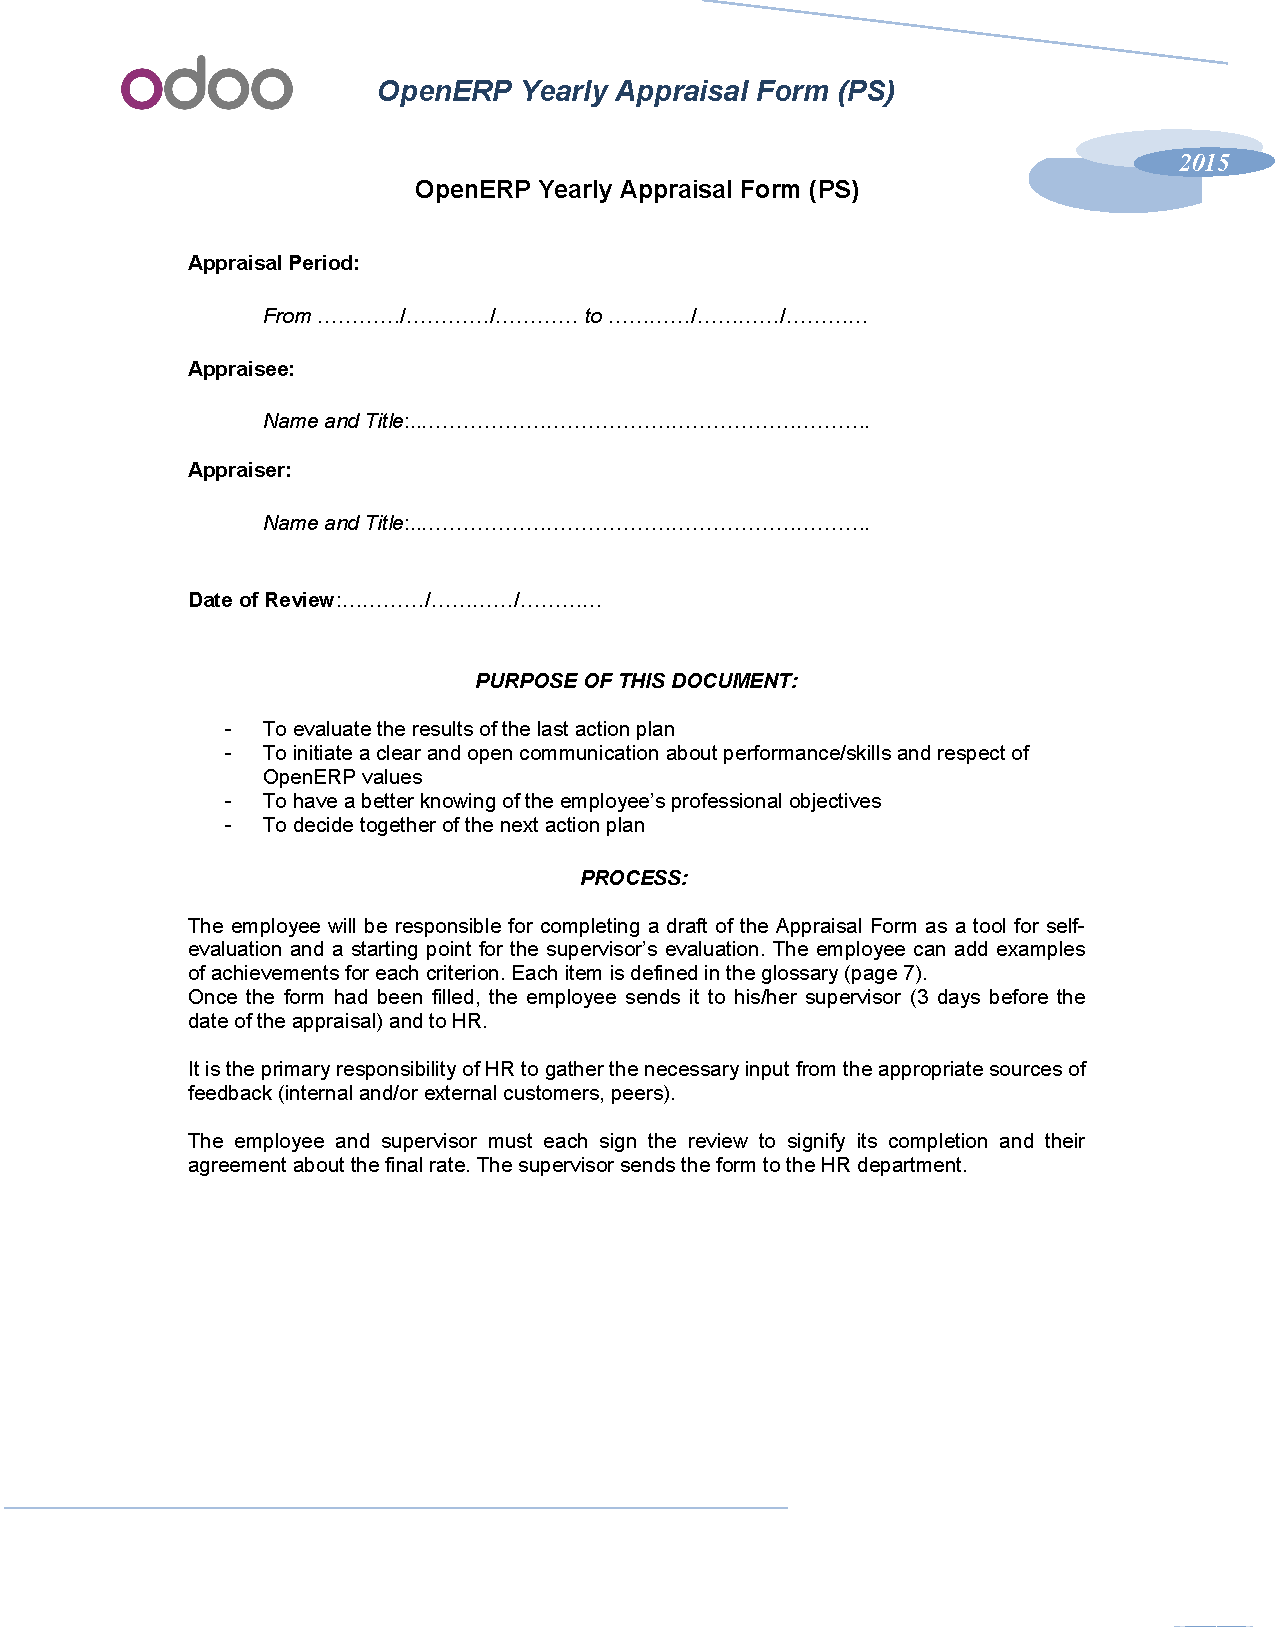
\includepdf[pages=1-6]{document/Odoo_appraisal.pdf}

\chapter{Processus d'élaboration d'un référentiel}

\begin{figure}[h!]
    \begin{center}
        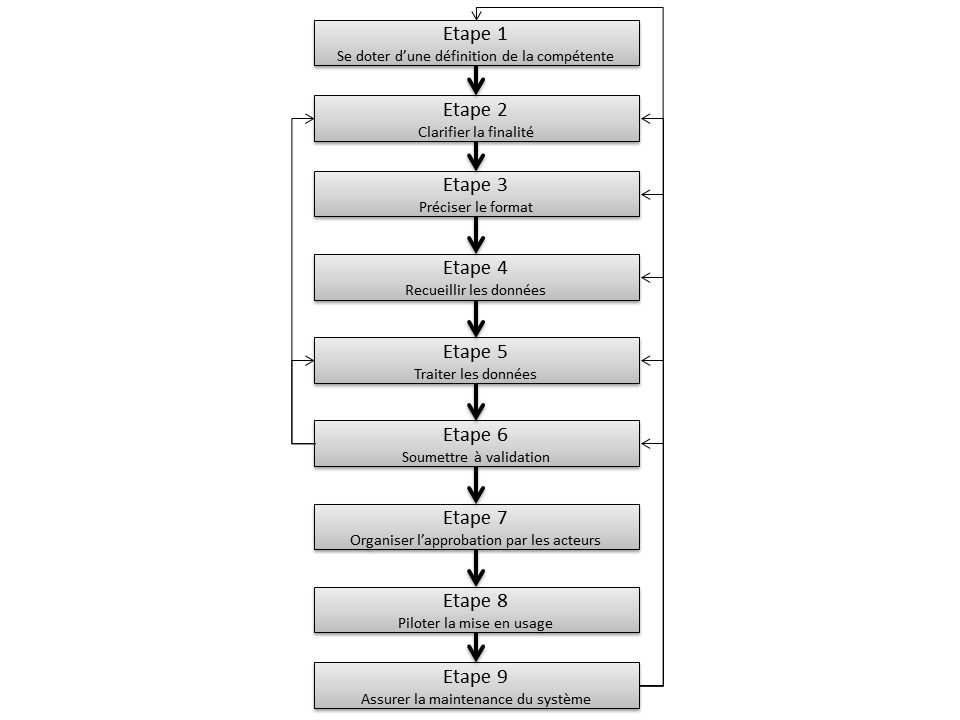
\includegraphics[scale=0.5]{document/process.png}
        \caption{Processus de l'élaboration et de la mise en service d'un référentiel de compétence. Source \citep[pp.41]{refcompetence} }
        \label{process}
    \end{center}
\end{figure}

\chapter{Ébauche du référentiel de compétences techniques}

\section{Processus à analyser}
\begin{description}
  \item[Projet]
  Gestion de projet du point de vue de l’équipe technique, de l'analyse technique à la maintenance en passant par les développements et les tests. L'un des processus les plus complexes à gérer mais aussi l'un des mieux maitriser et mieux documenter
  \item[Support Technique]
  Le processus est en soit assez simple mais relève de cas le plus souvent complexe et inédit. Il nécessite beaucoup d'ingéniosité mais aussi beaucoup de tact.
  \item[Formation]
  Le contenu de la formation est simple et relativement stable. Mais ce processus nécessite des compétences pédagogiques importantes
  \item[Consultance]
  C'est un processus fourre-tout qui nécessite une bonne dose d'improvisation parfois et un bon contact avec le client
  \item[Développement Saas] 
  Ce processus est le plus simple et est assez bien maitrisé. Mais les possibilités limités de l'environnement nécessite pas mal de créativité.
  \item[Avant-vente]
  Malgré ces aspects l'avant-vente est un des processus les plus avancés, il nécessite généralement de bien maitrisé tous les autres mais il faut en plus maitriser des aspects humains et tenir compte de considération économique.
  \item[Administration de l'infrastructure]
  Processus clairement définit mais qui nécessite des compétences très différentes de toutes les autres. 
\end{description}


\section{Analyse des tâches du processus: Projet}
\begin{description}
    \item[Développement backend]
    Cette tâche consiste le coeur de l'activité de l'équipe, il faut traduire les spécifications fonctionnelles en module Odoo. Les modules sont écrits en Python et en Xml. Cette tâche requiert beaucoup de compétence. D'abord des compétences analytiques. Il faut comprendre la spécification fonctionnelle, l'analyser pour pouvoir la modéliser. Il faut ensuite pouvoir écrire le code, le tester et le délivrer. L'écriture du code demande des connaissances du langage python, du Framework Odoo, du langage xml et qweb. Pour tester sont codes, ils pouvoir construire des scénarios représentatifs de la réalité et tester les cas limites susceptible d'arriver. Pour délivrer le code, il faut connaître les procédures de la gestion du projet et le système de gestion des sources : git. 
    \item[Analyse Technique, estimation et faisabilité]
    Cette tâche consiste à vérifier que les spécifications fonctionnelles sont réalisable techniquement et en combien de temps. Pour cela, il faut déjà pouvoir se faire une idée de la manière de réaliser la spécification pour pouvoir estimer les temps nécessaire à sa réalisation. Cette tâche nécessite des connaissances techniques assez générales pour identifier la partie spécifique qui sera impacter par les demandes des clients. Ensuite en fonction du domaine, cette tâche requiert les mêmes compétences que le développement backend ou frond end. Il faut aussi connaitre toutes les phases nécessaires à la production de la fonctionnalité. Une connaissance du domaine fonctionnelle en question permet de challenger la spécification et de pouvoir parfois proposer une meilleure solution. 
    \item[Test fonctionnel]
    Cette tâche n'est pas effectuée par l'équipe technique mais elle peut l'être. Elle consiste à tester manuellement un développement pour vérifier que celui-ci correspond bien à la spécification fonctionnelle et qu'aucune erreur n'est rencontrée. La tâche de test fonctionnelle nécessite de connaitre et de comprendre les spécifications fonctionnelles de la fonctionnalité implémentée. Il faut être capable de concevoir des scénarios généraux mais aussi les scénarios limites à tester. Finalement, il faut être capable de mettre en pratique les scénarios de tests. 
    \item[Test automatique backend]
    
    Cette tâche est fort similaire à la précédente à la différence qu'il faut écrire en code les scénarios de test pour que ceux-ci puisse être lancé et s'exécuter automatiquement, elle nécessite de comprendre les spécifications mais aussi le code, de concevoir des scénarios de test et ensuite de les implémenter dans le framework de test Odoo. 
    \item[Revue de la qualité du code]
    L'objectif de cette tâche est de se prononcer sur la qualité du code écrit. Est-il lisible, répond-il à la spécification, est-il performant et robuste et ensuite de donner un feedback constructif à la personne qui a écrit le code. Cette tâche est l'une des plus complexes et les plus complètes. Elle nécessite des très bonnes connaissances des langages qui sont impliqués dans le code à reviewer, du framework Odoo pour pouvoir proposer de meilleures solutions que celles utilisées. Il faut pouvoir se construire une image globale du code en lisant ligne par ligne. Finalement, il faut un certain tact pour exprimer son feedback. Il faut aussi avoir intériorisé les recommandations de codage d'Odoo (Odoo guidelines) pour vérifier que celle-ci sont respectées. 
    \item[Déploiement d'Odoo] Cette tâche consiste à déployer Odoo sur un serveur avec tout le code nécessaire, de paramétrer correctement tous les composants du déploiement. 
    Cette tâche requiert des connaissances très différentes des précédentes. Il faut savoir utiliser le système d'exploitation Linux en ligne de commande, être capable d'installer les dépendances d'Odoo, d'installer et paramétrer Postgresql. Il faut aussi maitriser git et le paramétrage d'Odoo. 
\end{description}

\subsection{Tâches non détaillées dans cette annexe}


\begin{itemize}
 \item Test automatique frontend
 \item Développement Front end
 \item Web Design
 \item Administration Postgresql
 \item Performance optimisation
 \item Méthode agile
 \item Gestion des sources
 \item Documentation Technique
 \item Documentation Fonctionnelle
 \item Support
 \item Migration de version 
 \item Migration des données existantes
 \item Intégration du code
\end{itemize}


\section{Description de compétence}
Voici la liste des compétences dérivées des tâches qui ont été détaillées dans la section précédente. 
\subsubsection{Savoir programmer en python}
La connaissance du parfait d'un langage est un travail de plusieurs années, mais ce n'est pas ce qui est demandé. Il faut pouvoir manipuler les principales structures de donnée, comprendre la documentation et être capable d'utiliser les bibliothèques nécessaires au développement après en avoir lu la documentation. 




\subsubsection{Connaître et pouvoir utiliser le framework Odoo}
Il faut savoir appliquer le contenu de la formation technique. Connaitre tous les types de champs, de vues. Connaitre comment implémenter des wizards, l'écriture de rapports dynamique. 
Il faut savoir comment rendre les formulaires dynamique, ajouter des contraintes au système. Cette compétences peux encore se découper en plusieurs sous compétences. 
\subsubsection{Être capable de concevoir des scénarios de tests sur base de spécifications}
Ici, il est important de comprendre la spécification pour concevoir des tests qui permettent de s'assurer que le système sera fonctionnel une fois que les utilisateurs vont l'utiliser réellement. 
\subsubsection{Savoir implémenter des scénarios de tests pour les automatiser dans le backend}
Cette compétence nécessite de connaître le python et le framework Odoo en plus de cela il faut connaître le frameword unittest2 ainsi que sont implémentation dans Odoo. L'utilisation de l’outil coverage est un plus. 

\subsubsection{Savoir écrire des requête SQL}
Pouvoir écrite des requête de sélection de donnée, de création, de mise à jours et de suppression. Pouvoir effectuer des jointures entre les tables. 


\subsubsection{Être capable de découper un problème en plusieurs sous problème}
Ceci est particulièrement utile en programmation. Il faut pouvoir découper un problème un plusieurs petit problème jusqu'à ce que le sous-problème puisse directement s'exprimer dans le langage de programmation utilisé. 
\subsubsection{Compréhension fonctionnelle d'un module métier}
Avoir une compréhension fonctionnelle d'un module métier consiste à connaître son but, avoir fait l'expérience d'un cas concret d'implémentation du module, de pouvoir le configurer et de connaitre ses principales fonctionnalités. On peut citer les principaux modules:
\begin{itemize}
 \item CRM
 \item Vente
 \item Gestion de stock
 \item Gestion de la production
 \item Achat
 \item Comptabilité 
 \item Comptabilité analytique
 \item Marketing
 \item Point de vente
 \item Gestion de projet
 \item Gestion des ressources humaines
 \item Website
 \item E-commerce
\end{itemize}



\subsection{Compétence non détaillées dans cette annexe}
\begin{itemize}
 \item Connaitre et appliquer les guidelines odoo en programmation
 \item Savoir Programmer en javascript
 \item Savoir Programmer en bash
 \item Savoir écrire des fichiers xml odoo et des vues backend
 \item Savoir écrire des vues qweb
 \item Être capable d'administrer un serveur Postgresql
 \item Être capable d'administrer un serveur linux
 \item Pouvoir adapter son discours en fonction de son interlocuteur
 \item Être capable d'utiliser l'outil de gestion de sources git
 \item Connaître et appliquer les procédures mis en place pour la bonne marche du projet
 \item Être capable de communique de manière sereine et constructive son feedback
 \item Être capable d'estimer le temps nécessaire à une tâche de programmation
 \item Pouvoir lire et comprendre le code d'autrui et pouvoir en extraire le sens
 \item Être capable de déployer et d'administrer Odoo
 \item Être capable de traduire les spécifications dans un modèle technique et d'en découler les tâches techniques à réaliser
 
\end{itemize}


\section{Exemple de socle de base}
On pourrait imaginer un socle de base qui requiert de pouvoir effectuer les tâches suivantes de manière autonome : développement backend; test fonctionnel; Test automatique backend; déploiement d'Odoo.
Il faudrait pour cela avoir une maitrise de niveau 3 des compétences suivantes. 
\begin{itemize}
 \item Être capable de traduire les spécifications dans un modèle technique et d'en découler les tâches techniques à réaliser
 \item Être capable de découper un problème en plusieurs sous problème
 \item Savoir programmer en python
 \item Connaître et pouvoir utiliser le framework Odoo
 \item Savoir écrire des fichiers xml odoo et des vues backend
 \item Être capable de déployer et d'administrer Odoo
 \item Savoir implémenter des scénarios de tests pour les automatiser dans le backend
 \item Être capable de concevoir des scénarios de tests sur base de spécifications
 \item Compréhension fonctionnelle de 2 modules
\end{itemize}


\section{Exemple de profil cohérent}
\subsection{Profil : Développeur Backend}
\begin{itemize}
 \item Connaitre le framework Odoo
 \item Être capable de modifier des modules Odoo existant
 \item Être capable d'étendre des modules Odoo existant
 \item Être capable créer des nouveaux modules
 \item Savoir programmer en python
 \item Savoir écrire des requête SQL
 \item Savoir écrire des fichiers xml odoo et des vues backend
 \item Connaitre les outils de débogage python
 \item Savoir implémenter des tests automatisés pour le backend par rapport au périmètre de son propre code
 \item Connaitre les guideline de développement Odoo
 \item Connaissance de git
 \item Connaissance technique des modules de base: Base, Email

\end{itemize}




\end{document}
